\documentclass[11pt,twoside,a4paper]{book}  
% definice dokumentu
\usepackage[czech, english]{babel}
\usepackage[T1]{fontenc} 				% pouzije EC fonty 
\usepackage[utf8]{inputenc} 			% utf8 kódování vstupu 
\usepackage[square, numbers]{natbib}	% sazba pouzite literatury
\usepackage{indentfirst} 				% 1. odstavec jako v~cestine, pro práci v~aj možno zakomentovat
\usepackage{fancyhdr}					% tisk hlaviček a~patiček stránek
\usepackage{nomencl} 					% umožňuje snadno definovat zkratky a~jejich seznam

%%%%%%%%%%%%%%%%%%%%%%%%%%%%%%%%%%%%%%%%%%%%%%%%%%%%%%%%%%%%%%%
% informace o práci
\newcommand\WorkTitle{Software pro distribuované řízení a vyčítání dat ze sítě částiových pixelových detektorů Timepix3} % název
\newcommand\FirstandFamilyName{Bc. Jakub Begera} % autor
\newcommand\Supervisor{Ing. Štěpán Polanský} % vedoucí

\newcommand\TypeOfWork{Diplomová práce}	% typ práce [Diplomová práce | Bakalářská práce | Bachelor's Project | Master's Thesis ]	

% Nastavte následují podle vašeho oboru a~programu (pomoc hledejte na http://www.fel.cvut.cz/cz/education/bk/prehled.html)								
\newcommand\StudProgram{Otevřená informatika} % program
\newcommand\StudBranch{Softwarové inženýrství} % obor

%%%%%%%%%%%%%%%%%%%%%%%%%%%%%%%%%%%%%%%%%%%%%%%%%%%%%%%%%%%%%%%
% minimální importy
\usepackage{graphicx}					% pro vkládání obrázků
\usepackage{k336_thesis_macros} 		% specialni makra pro formatovani DP a~BP
\usepackage[
pdftitle={\WorkTitle},				% nastaví v~informacích o pdf název
pdfauthor={\FirstandFamilyName},	% nastaví v~informacích o pdf autora
colorlinks=true,					% před tiskem doporučujeme nastavit na false, aby odkazy a~url nebyly šedé při ČB tisku
breaklinks=true,
urlcolor=red,
citecolor=blue,
linkcolor=blue,
unicode=true,
]
{hyperref}								% pro zobrazování "prokliknutelných" linků 

% rozšiřující importy
\usepackage{listings} 			%slouží pro tisk zdrojových kódů se syntax higlighting
\usepackage{algorithmicx} 		%slouží pro zápis algoritmů
\usepackage{algpseudocode} 		%slouží pro výpis pseudokódu
\usepackage{inconsolata}		%monospace font
\usepackage{soul}				%zvýrazňovač
\usepackage[final]{pdfpages}    %PDF include
\usepackage{subcaption}			%pro reference na subfigures 
\usepackage{enumitem}
\usepackage{bytefield}
\usepackage{pgf-umlsd}			%sekvenční UML diagramy
\usepackage{tikz}		        %TeX obrázky
\usetikzlibrary{trees,calc,positioning,shapes.geometric,matrix,arrows,decorations.pathreplacing,arrows.meta,decorations.markings,math}

\usepackage{minted}				% slouží k~Syntax Highlighting
\usepackage{amsmath}

\usepackage{forest}
\definecolor{folderbg}{RGB}{124,166,198}
\definecolor{folderborder}{RGB}{110,144,169}
\definecolor{cvut_color}{RGB}{3,46,85}
\definecolor{blue_ligh}{RGB}{0,118,203}

\def\Size{4pt}
\tikzset{
  folder/.pic={
    \filldraw[draw=folderborder,top color=folderbg!50,bottom color=folderbg]
      (-1.05*\Size,0.2\Size+5pt) rectangle ++(.75*\Size,-0.2\Size-5pt);  
    \filldraw[draw=folderborder,top color=folderbg!50,bottom color=folderbg]
      (-1.15*\Size,-\Size) rectangle (1.15*\Size,\Size);
  }
}

%%%%%%%%%%%%%%%%%%%%%%%%%%%%%%%%%%%%%%%%%%%%%%%%%%%%%%%%%%%%%%%
% příkazy šablony
\makenomenclature								% při překladu zajistí vytvoření pracovního souboru se seznamem zkratek
% zkratky CERN + ČVUT
\nomenclature{CERN}{Evropská organizace pro jaderný výzkum (Originální název: \textit{Conseil Européen pour la Recherche Nucléaire}), se sídlem v Ženevě, ve Švýcarsku.}
\nomenclature{ATLAS}{A Toroidal LHC Apparatus}
\nomenclature{LHC}{Large Hadron Collider}
\nomenclature{LS}{Long Shutdown - dlouhodobá technologická přestávka LHC}
\nomenclature{DCS}{Detector Control Systems}
\nomenclature{DSS}{Detector Safety System}
\nomenclature{DAQ}{Data Acquisition System}
\nomenclature{ÚTEF}{Ústav technické a experimentální fyziky}
\nomenclature{SATRAM}{Space Application of Timepix based Radiation Monitor}

% detektory
\nomenclature{TPX}{Timepix}
\nomenclature{MPX}{Medipix}
\nomenclature{TOT}{Time Over Treshold - mód detektoru (viz \ref{det:mod})}
\nomenclature{ToA}{Time of Arrival - mód detektoru (viz \ref{det:mod})}
\nomenclature{ASIC}{Application-specific Integrated Circuit}
\nomenclature{FPGA}{Field Programmable Gate Array}
\nomenclature{DAC}{Digitálně analogový převodník}
\nomenclature{ADC}{Analogově digitální převodník}
\nomenclature{CMOS}{Complementary Metal Oxide Semiconductor}
\nomenclature{CSM}{Charge Summing Mode}
\nomenclature{FITPix}{Fast Interface for Timepix Pixel Detectors}
\nomenclature{LVDS}{Low-voltage differential signaling}
\nomenclature{PCC}{Photon Counting Chip}
\nomenclature{ISO}{International Organization for Standardization}
\nomenclature{OSI}{Open Systems Interconnection model}

% software & hardware & elektronika
\nomenclature{HTTPS}{Hypertext Transfer Protocol Secure}
\nomenclature{HTTP}{Hypertext Transfer Protocol}
\nomenclature{API}{Application Programming Interface}
\nomenclature{REST}{Representational State Transfer}
\nomenclature{JSON}{JavaScript Object Notation}
\nomenclature{SQL}{Structured Query Language}
\nomenclature{URL}{Uniform Resource Locator}
\nomenclature{b}{bite}
\nomenclature{B}{byte}
\nomenclature{PC}{Personal Computer}
\nomenclature{HW}{Hardware}
\nomenclature{SW}{Software}
\nomenclature{USB}{Universal Serial Bus}
\nomenclature{PN}{Přechod polovodiče typu P a polovodiče typu N}
\nomenclature{TCP}{Transmission Control Protocol}
\nomenclature{IP}{Internet Protocol}
\nomenclature{SSH}{Secure Shell}
\nomenclature{PCB}{Printed Circuit Board}
\nomenclature{SPI}{Serial Peripheral Interface}
\nomenclature{GPIO}{General Purpose Input/Output}
\nomenclature{UDP}{User Datagram Protocol}
\nomenclature{SFTP}{Secure File Transfer Protocol}
\nomenclature{HDFS}{Hadoop Distributed File System}
\nomenclature{DOM}{Document Object Model}
\nomenclature{DSL}{Domain-specific language}
\nomenclature{J2EE}{Java Enterprise Edition}
\nomenclature{JPA}{Java Persistent API}
\nomenclature{JAR}{Java Archive}
\nomenclature{WAR}{Web Application Archive}
\nomenclature{BSON}{Binární forma JSON}
\nomenclature{JSON}{JavaScript Object Notation}
\nomenclature{REST}{Representational State Transfer}
\nomenclature{ID}{Identifikátor}
\nomenclature{LOB}{Large Object}
\nomenclature{CRUD}{Create, read, update and delete}
\nomenclature{HTML}{Hypertext Markup Language}
\nomenclature{MVC}{Model View Controller}
\nomenclature{ACQ}{Datagram typu acknowledge}
\nomenclature{ASCII}{American Standard Code for Information Interchange}
\nomenclature{UTC}{Koordinovaný světový čas (anglicky Coordinated Universal Time)}
\nomenclature{ORM}{Object-relational mapping}
\nomenclature{JRE}{Java Runtime Environment}
\nomenclature{CSS}{Cascading Style Sheets}
\nomenclature{JS}{JavaScript}

% matematické zkratky
\nomenclature{FWHM}{Full width at half maximum}

% fyzikální a chemické zkratky
\nomenclature{eV}{elektronvolt}
\nomenclature{GaAs}{Arsenid gallitý}
\nomenclature{CdTe}{Cadmium telluride}
\nomenclature{Si}{Křemík}
\nomenclature{In}{Indium}
\nomenclature{Fe}{Železo}
\nomenclature{Cu}{Hliník}


\let\oldUrl\url									% url adresy budou zobrazeny: <url> 
\renewcommand\url[1]{<\texttt{\oldUrl{#1}}>}
%\renewcommand\lstlistingname{Výpis kódu} % předefinování nadpisu
%\renewcommand\lstlistlistingname{Výpisy kódu} % předefinování nadpisu v~obsahu
%\renewcommand{\lstlistingname}{Algorithm}% Listing -> Algorithm
%\renewcommand{\lstlistlistingname}{Listdassad of \lstlistingname s}% List of Listings -> List
%%%%%%%%%%%%%%%%%%%%%%%%%%%%%%%%%%%%%%%%%%%%%%%%%%%%%%%%%%%%%%%
% vaše vlastní příkazy
\newcommand*{\nomExpl}[2]{#2 (#1)\nomenclature{#1}{#2}} % usnadňuje zápis zkratek : Slova ke Zkrácení (SZ)
\newcommand*{\nom}[2]{#1\nomenclature{#1}{#2}} % usnadňuje zápis zkratek : SZ
\newcommand*{\todo}{\hl{\textbf{TODO}}} % pro poznámky
\newcommand{\addbibresource}[1]{}
\newcommand*{\footnoteUrl}[1]{\footnote{\url{#1}}}
\newcommand{\unit}[2]{$#1~\ensuremath{\mathrm{#2}}$} % pro jednotky

% custom padding
\def\changemargin#1#2{\list{}{\rightmargin#2\leftmargin#1}\item[]}
\let\endchangemargin=\endlist 

\usepackage{caption}
\DeclareCaptionType{code}[Zdrojový kód][Seznam zdrojových kódů] 
%%%%%%%%%%%%%%%%%%%%%%%%%%%%%%%%%%%%%%%%%%%%%%%%%%%%%%%%%%%%%%%
% vlastní dokument
%%%%%%%%%%%%%%%%%%%%%%%%%%%%%%%%%%%%%%%%%%%%%%%%%%%%%%%%%%%%%%%
\begin{document}

	%%%%%%%%%%%%%%%%%%%%%%%%%% 
	% nastavení jazyka, kterým je práce psána
	\selectlanguage{czech}	% podle jazyka práce nastavte na [czech | english]
	\translate				% nastaví české nebo anglické popisy (např. katedra -> department); viz k336_thesis_macros


	%%%%%%%%%%%%%%%%%%%%%%%%%%    
	% Titulni stranka / Title page 
	\coverpagestarts

	%%%%%%%%%%%%%%%%%%%%%%%%%%    
	% Zadani / Assignment
	\newpage~
	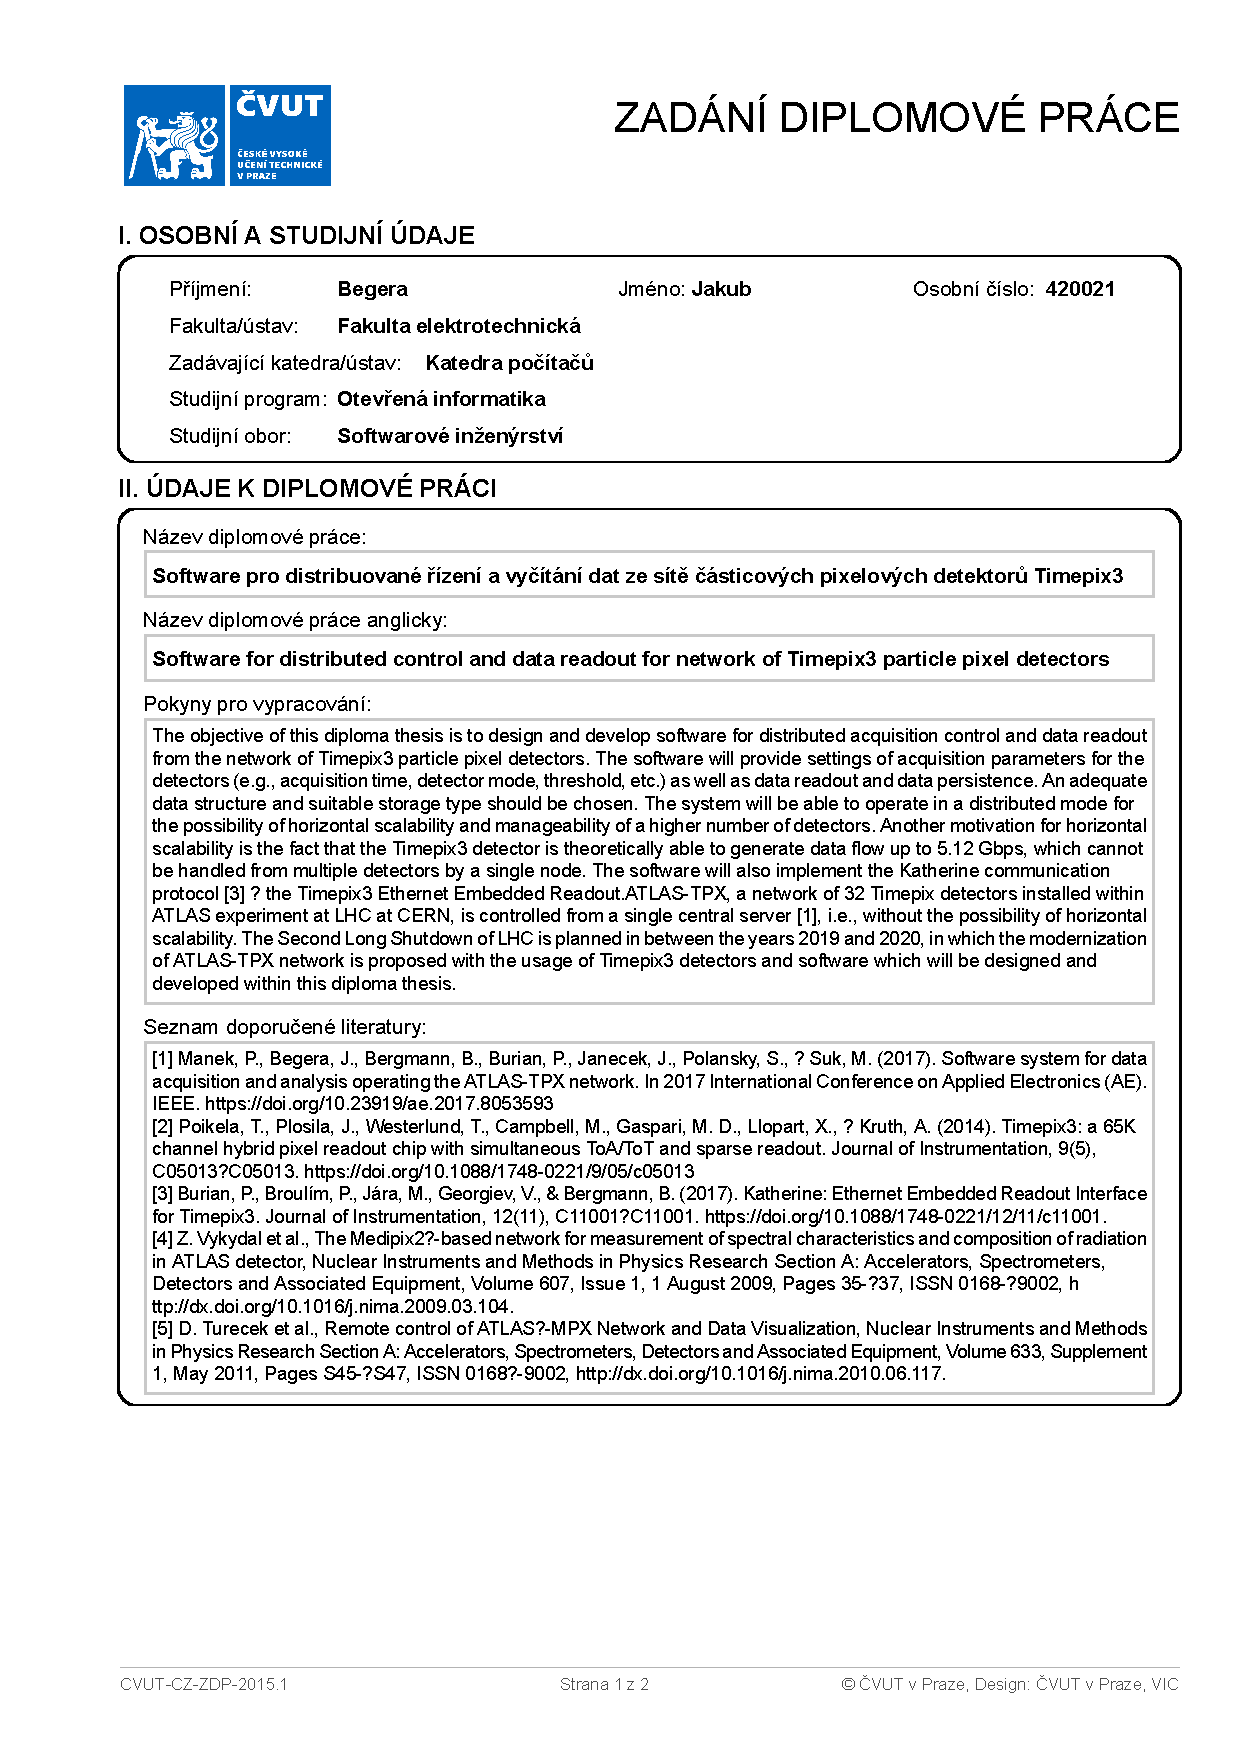
\includepdf[pages=1,pagecommand={},offset=0cm -3cm]{zadani.pdf}
	\includepdf[pages=2,pagecommand={},offset=0cm -3cm]{zadani.pdf}
	\newpage

	%%%%%%%%%%%%%%%%%%%%%%%%%%%    
	% Poděkovani / Acknowledgements 
	\acknowledgements
	\noindent
	\todo


	%%%%%%%%%%%%%%%%%%%%%%%%%%%   
	% Prohlášení / Declaration 

	\declaration{V~Praze dne 27.\,5.\,2016}


	%%%%%%%%%%%%%%%%%%%%%%%%%%%%    
	% Abstrakt / Abstract 
 
	\abstractpage

	\todo abstrakt anglicky

	
	\vglue60mm
	\noindent{\Huge \textbf{Abstrakt}}
	\vskip 2.75\baselineskip

	\todo abstrakt česky


	%%%%%%%%%%%%%%%%%%%%%%%%%%    
	% obsahy a~seznamy
	\tableofcontents		% Obsah
	\listoffigures			% Seznam obrázků
	\listoftables			% Seznam tabulek
	\listofcodes			% Seznam zdrojových kódů	

	%%%%%%%%%%%%%%%%%%%%%%%%%% 
	% začátek textu  
	\mainbodystarts

\addbibresource{reference.bib}

\chapter{Introduction}\label{chap01}
Test
\addbibresource{reference.bib}

\chapter{Úvod do hybridních částicových pixelových detektorů}\label{chap:detectors}
Ionizující záření je lidskými smysli nedetekovatelné, avšak jeho studie nám umožňuje pochopit podstatu hmoty, její vlastnosti a interakce. To lidstvu umožnilo mnohé aplikace, jako je například protonová terapie \cite{tpx_app_radiotherapy}, defektoskopie nebo zkoumání pravosti uměleckých děl. První pokusy o detekci ionizujícího záření sahají do počátku 20. století, kde pomocí mlžné komory se prvně podařilo zachytit trajektorii nabitých částic. Rozvoj polovodičové technologie dal vzniku novým detekčním technologiím až po v současné době nejpokrokovějším - pixelovým detektorům.

Existuje celá řada částicových pixelových detektorů, ale v této kapitole budou popsány jen hybridní pixelové detektory, pro které je typické, že se skládají ze dvou nezávisle vyrobených částí - senzoru a vyčítacího čipu. To oproti monolitickým detektorů, kde vyčítací elektronika je součástí senzoru přináší řadu výhod, jako například snížení výrobních nákladů nebo možnost kombinace vyčítacího čipu se senzory různých materiálů (\textit{Si}, \textit{GaAs}, \textit{CaTe} apod.) a tlouštěk (vetšinou $300\mu m$, nebo $500\mu m$).

Na tomto místě je třeba zmínit, že existuje více druhů těchto detektorů (\textit{AGH Fermilab, Pilatus, Philips Chromaix} apod.)\cite{detectors_review}, v této práci budou použity použity pouze detektory z rodiny detektorů Medipix.

%********************************************************************************
% Hardwarová architektura
%********************************************************************************
\section{Hardwarová architektura}
\begin{figure}[th]
	\begin{center}
		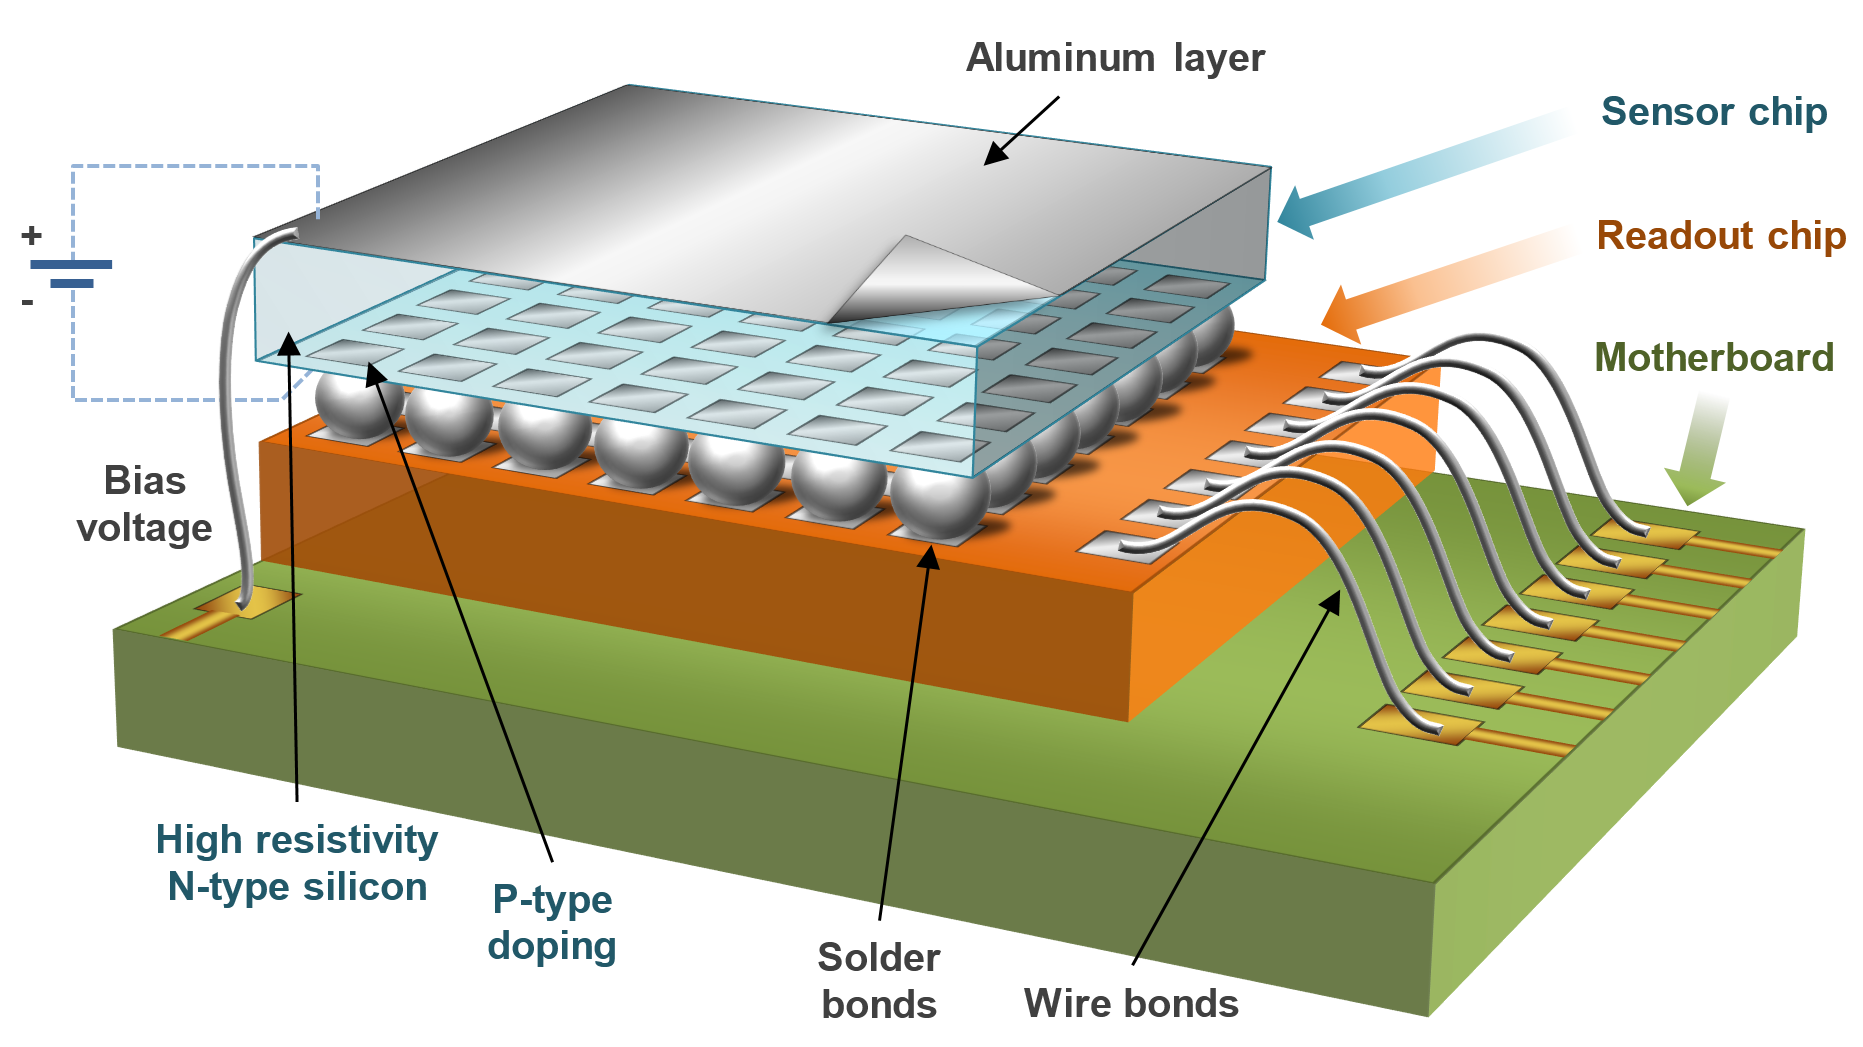
\includegraphics[width=12cm]{figures/det_chip.png}
		\caption{Struktura hybridního polovodičového pixelového detektoru Timepix3, skládající se z vyčítacího čipu a polovodičového senzoru \cite{PlatkevicDisertace}.}
		\label{fig:det:chip}
	\end{center}
\end{figure}
Většina hybridních částicových pixelových detektorů rodiny Medipix obsahuje matici $256\times256$ pixelů. Každý z nich má stanu o délce $55~\mu m$, takže senzor čítající $65536$ má plochu $1.4 \times 1.4 cm^2$. 

Na obrázku \ref{fig:det:chip} je znázorněna struktura detektoru Timepix3. Vrchní část detektoru tvoří polovodičový senzor, který je nejčastěji vyroben z křemíku, ale výjimkou není také \textit{GaAs} nebo \textit{CaTe}. Jednotlivé pixely senzoru jsou spojeny s integrovaným \texttt{ASIC}\footnote{z angl. Application Specific Integrated Circuit} vyčítacím čipem pomocí technologie zvané \textit{Bump-Bounding}. Vyčítací čip je pak propojen se základní deskou pomocí \textit{wire-bound}, z které je ještě přivedeno měřící napětí na senzor detektoru (tzv. \textit{bias}).


%********************************************************************************
% Princip detekce
%********************************************************************************
\section{Princip detekce}\label{chap:detectors:princip}
\begin{figure}[th]
	\begin{center}
		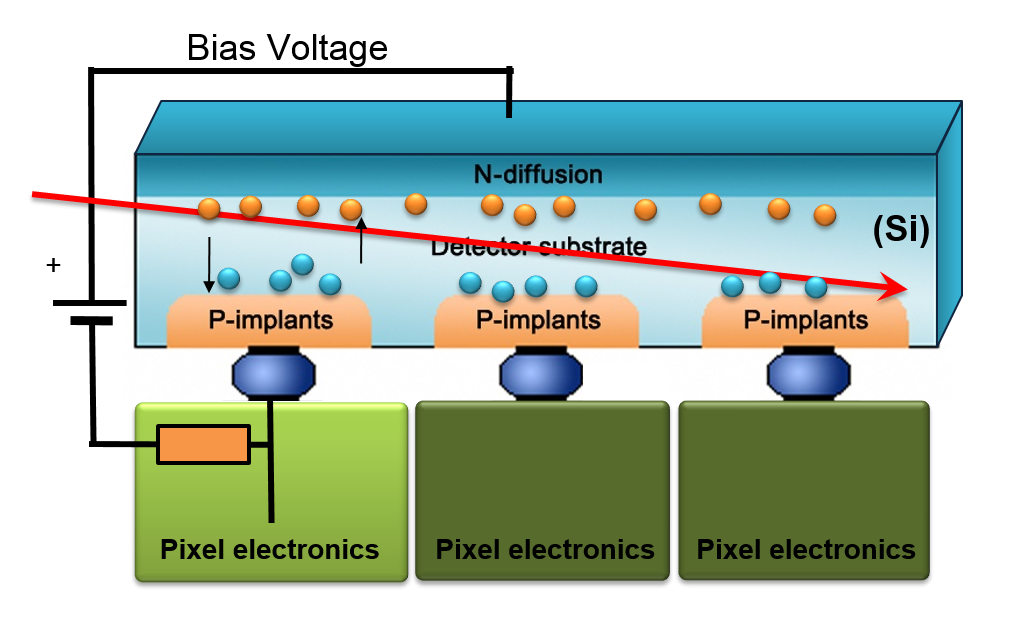
\includegraphics[width=10cm]{figures/det_recombination.png}
		\caption{Princip detekce ionizujícího záření detektorem Timepix3 \cite{PlatkevicDisertace}.}
		\label{fig:det:recombination}
	\end{center}
\end{figure}

Princip detekce ionizujícího záření pixelovými detektory je založen na známém jevu detekce ionizujícího záření v polovodiči. 

Jako náhradní schéma jednoho pixelu si lze představit diodu zapojenou v závěrném směru, kterou bez přítomnosti ionizujícího záření protéká minimální proud. Vnikne-li do senzoru ionizující částice a dojde k její interakci se senzorem, resp. část její energie je deponována do polovodičového objemu senzoru, dojde v senzoru ke vzniku elektron-děrových páru a díky lavinovému efektu i k následnému otevření PN přechodu (viz. na obr. \ref{fig:det:recombination}, kde červená šipka znázorňuje interagující částici, elektrony jsou znázorněny žlutě, modře díry).

Vzniklý proudový impulz je měřícím odporem převeden na napětí, které je komparátorem porovnáno s prahovým napětím (tzv. \textit{threshold}). Výsledek této komparace je dále CMOS obvodem zpracován, dle použitého měřícího módu, jak bude ukázáno v kapitole \ref{chap:detectors:operation_modes}.

Na rozdíl od CCD technologii, CMOS readout \textit{Timepix}/\textit{Medipix} detektorů negeneruje temný proud\footnote{Termín charakterizující vyčítací šum u CCD snímačů. Obvykle je udáván v elektronech za sekundu při konstantní teplotě a ve tmě.}, díky odstínění signálu od šumu pomocí komparačního napětí. To znamená, že doba jedné akvizice je teoreticky neomezena, protože detektor je schopný detekovat jen ty částice, jejíchž deponovaná energie (resp. amplituda vzniklého napěťového pulzu) je větší, než \textit{threshold}.

%********************************************************************************
% Operační módy detektoru
%********************************************************************************
\section{Operační módy detektoru}\label{chap:detectors:operation_modes}
\begin{figure}[th]
	\begin{center}
		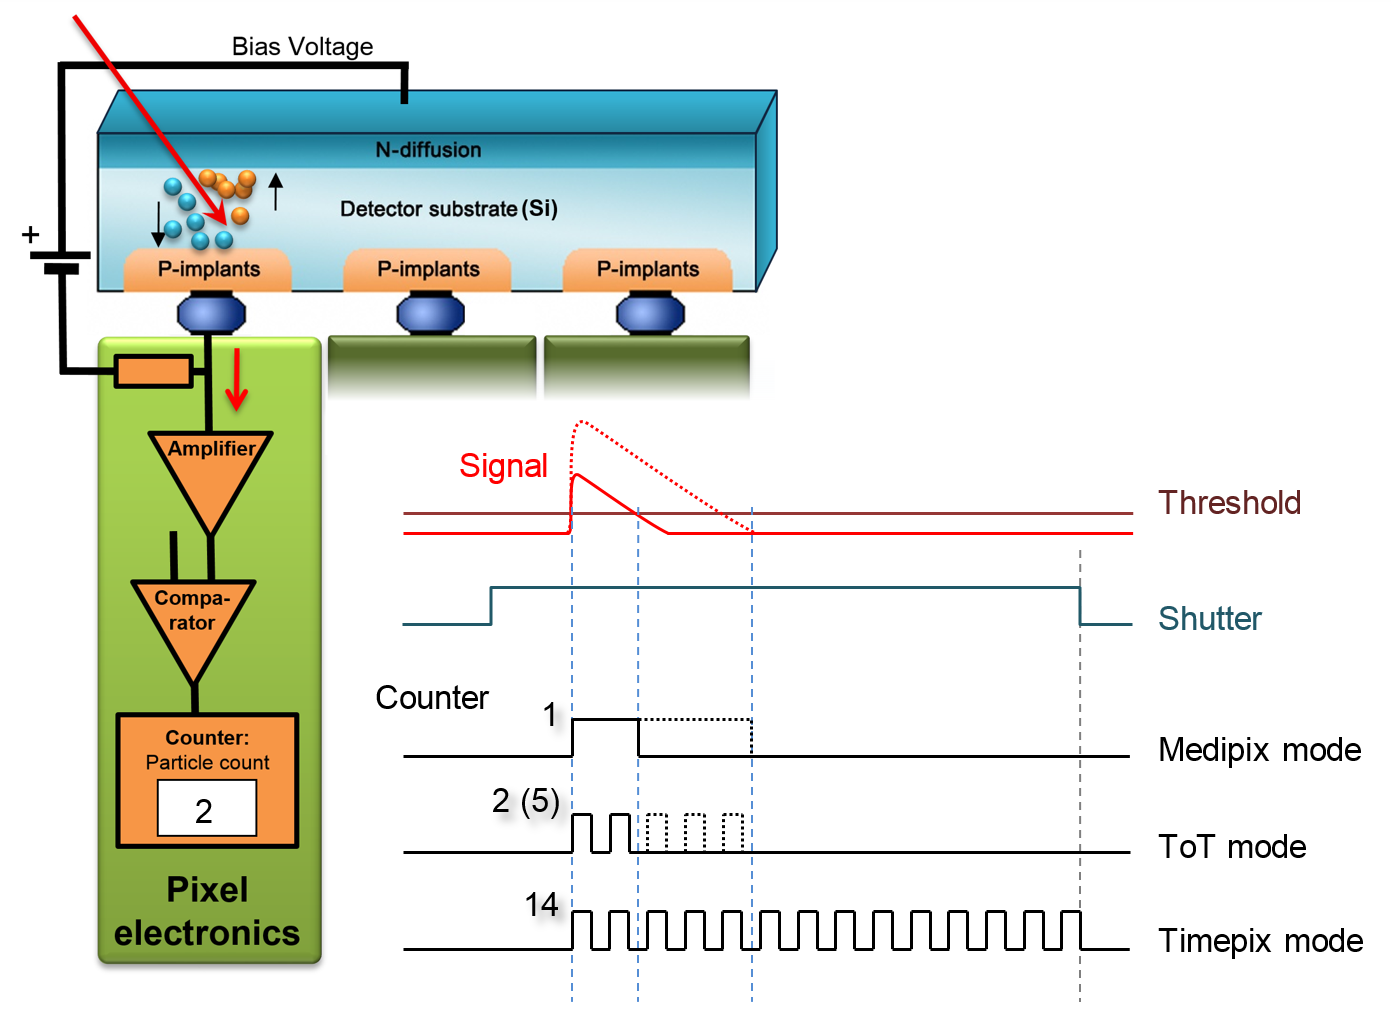
\includegraphics[width=14cm]{figures/det_pix.png}
		\caption{Zpracování signálu pixelem detektoru dle nastaveného módu (\textit{Medipix}, \textit{ToT} a \textit{ToA}) \cite{PlatkevicDisertace}.}
		\label{fig:det:modes}
	\end{center}
\end{figure}


V této podkapitole bude vysvětlena většina operačních módu, ve kterých detektory rodiny \textit{Medipix} jsou schopny pracovat. 

Jak už bylo popsáno v předchozí kapitole, interagovaná částice vyvolá napěťový impulz, jehož tvar koreluje s deponovanou energií. Pro účely analýzy se ale používá pouze binární informace o překročení prahového napětí v čase. Výsledek této analýzy je po jejím dokončení uložen ve 14-bitovém registru pixelu.

Na obr. \ref{chap:detectors:operation_modes} je znázorněn příklad zpracování analýzy signálu následujícími módy:
\begin{description}
    \item[Medipix mód (Counting mód)] V tomto módu je čítač inkrementován v každém cyklu měřící frekvence, pokud měřící napětí překročilo prahové napětí pixelu. Na konci akvizice pak hodnota čítače odpovídá počtu zaznamenaných částic.
    \item[Time-Over-Threshold (ToT)] Pracuje-li pixel v tomto módu, pak jeho čítač je inkrementování v každém cyklu měřící frekvence, pokud měřící napětí je vyšší, než prahové napětí pixelu. Hodnota uložená v čítači odpovídá deponované energii interagovaných částic. Mezi energií a \texttt{ToT} je nelineární závislost a její zkoumání je předmětem energetické kalibrace detektoru, jak bude ukázáno v kapitole \ref{chap:detectors:calibration:energy}. Tento mód má široké spektrum aplikací, například \cite{tot_app_counting} nebo \cite{tpx_app_radiotherapy}.
    \item[Time-of-Arrival (ToA)] Tímto módem disponují pouze detektory \textit{Timepix} a \textit{Timepix3}, avšak nesdílí stejný princip. Zatímco \textit{Timepix} detektor začne inkrementovat čítač v každém cyklu měřící frekvence po první náběžné hraně z komparátoru, \textit{Timepix3} na náběžnou hranu uloží do 14-bitového registru aktuální časové razítko z hodin detektoru. V obou případech \texttt{ToA} udává čas první interakce částice v dané akvizici.
\end{description}

%********************************************************************************
% Vyčítání naměřených dat
%********************************************************************************
\section{Vyčítání naměřených dat}\label{chap:detectors:readout}
Jednotlivé detektory rodiny \textit{Medipix} mají různou hardwarovou podporu pro vyčítání naměřených dat. Detektory vždy podporují alespoň jeden z těchto módů:
\begin{description}
	\item[Frame-Based] Pracuje-li detektor v tomto módu, pak jsou všechny registry čítačů pixelů vyčítány najednou, po dokončení aktuálního snímku. Vždy je třeba vyčíst všechny pixely bez ohledu na naměřenou hodnotu.
	\item[Data-Driven] Tento mód, také označovaný jako \textit{Event-Driven}, byl prvně použit v detektoru \textit{Timepix3}. Pracuje-li detektor v tomto módu, pak v průběhu akvizice dat (resp. když \textit{shutter} signál na nastaven na úroveň \texttt{HIGH}) každý pixel po zpracování události notifikuje readout interface o tom, že nová data jsou připravena k vyčtení a readout interface je pak bez prodlení vyčte a dále zpracuje.
\end{description}

Na obrázku \ref{fig:det:frame_vs_event_driven} je vidět hlavní motivace pro zavedení podpory \textit{Data-Driven} módu u detektoru \textit{Timepix3}. Ukázalo se, že \textit{Data-Driven} mód je efektivnější při takových měření, kde okupance snímků je menší než zhruba $50\%$. Po překročení této meze je efektivnější použití \textit{Frame-Based} módů, protože není třeba přenášet souřadnice zasažených pixelů. Podle \cite{timepix3} vyčítací čas může být definován následovně:
\begin{equation}\label{eq:det:readout_time}
	T_{readout} = N_{pixels}*bits_{pixel}/BW
\end{equation}
kde:
\begin{changemargin}{1.5cm}{1cm} 
	\begin{itemize}
		\item[$N_{pixels}$] je počet pixelů které je potřeba vyčíst (pro \textit{Frame-Based} mód jsou to všechny pixely detektoru ($256\times256$) a pro \textit{Data-Driven} je to počet zasažených pixelů),
		\item[$bits_{pixel}$] je počet bitů na pixel ($28 b$ v \textit{Frame-Based} módu a $28b + 16b$ v \textit{Data-Driven} módu kvůli nutnosti přenášení adresy pixelu) a
		\item[$BW$] je počet bytů za vteřinu, které je možné vyčíst z detektoru (\textit{bandwidth}). 
	\end{itemize}
\end{changemargin}

\begin{figure}[th]
	\begin{center}
		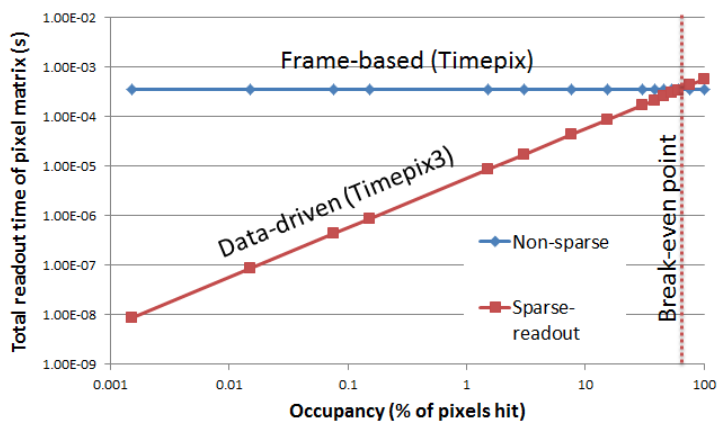
\includegraphics[width=14cm]{figures/det_frame_vs_event_driven.png}
		\caption{Doba vyčítání detektoru za použití \textit{Frame-based} (non-sparse) a \textit{Data-driven} (sparse) módu \cite{timepix3}.}
		\label{fig:det:frame_vs_event_driven}
	\end{center}
\end{figure}

%********************************************************************************
% Kalibrace
%********************************************************************************
\section{Kalibrace}\label{chap:detectors:calibration}
Každý detektor má své specifické vlastnosti, které jsou dány nejenom výrobním procesem, ale i závislostí na opotřebení a únavě materiálu v čase, okolní teplotě nebo na nastavených měřících parametrech (například \textit{bias}). Hlavní motivací pro kalibraci detektorů je minimalizace systematické chyby měření. Z pohledu aplikace získaných kalibračních dat je možné kalibrační metody rozdělit do dvou kategorií:
\begin{enumerate}[label=(\roman*)]
	\item Použití v průběhu akvizice dat - jedná se o data, která jsou použita pro nastavení akvizice dat v detektoru a mají přímý vliv na naměřená data, která danou metodou není možné dodatečně kalibrovat. Do této kategorie spadá například \textit{treshold equalizace} (viz \ref{chap:detectors:calibration:equalization}).
	\item Transformace naměřených dat - v tomto případě jsou kalibrační data aplikovaná dodatečně na naměřená data. Tento přístup má výhodu v možnosti dodatečné kalibrace již naměřených dat. To této kategorie spadá například \textit{Energetická kalibrace} (viz \ref{chap:detectors:calibration:energy}) nebo \textit{Time-Walk korekce} (viz \ref{chap:detectors:calibration:timeWalk}).
\end{enumerate}

\subsection{Treshold equalizace}\label{chap:detectors:calibration:equalization}
V podkapitole \ref{chap:detectors:princip} a \ref{chap:detectors:operation_modes} již bylo vysvětleno použití prahového napětí (\textit{treshold}) v průběhu akvizice dat detektorem. Každý pixel detektoru má ale rozdílné fyzikální vlastnosti dané výrobním procesem, s čímž souvisí i citlivost (resp. oddělení užitečného signálu od šumu) jednotlivých pixelů. Kromě globální hodnoty tresholdu je možné pro každý pixel upravit citlivost pomocí lokální $4b$ hodnoty tresholdu (viz obr. \ref{fig:det:medipix_overview:timepix3_schema}).

Vlastní proces equalizace probíhá tak, že se udělá treshold scan přes všechny hodnoty, přičemž je třeba minimalizovat interakce detektoru z částicemi. V běžné praxi stačí detektor dostatečně odstínit. Výstupem tohoto procesu je pak globální treshold a jeho 4-bitové korekce pro jednotlivé pixely.

Jako vedlejší produkt tohoto procesu je rovněž maskovací matice detektoru, které obsahuje šumějící, nebo jinak poškozené pixely. To jsou například takové pixely, které bez přítomnosti interagujících částic hlásí překročení tresholdu.

\subsection{Energetická kalibrace}\label{chap:detectors:calibration:energy}
\begin{figure}[th]
	\begin{center}
		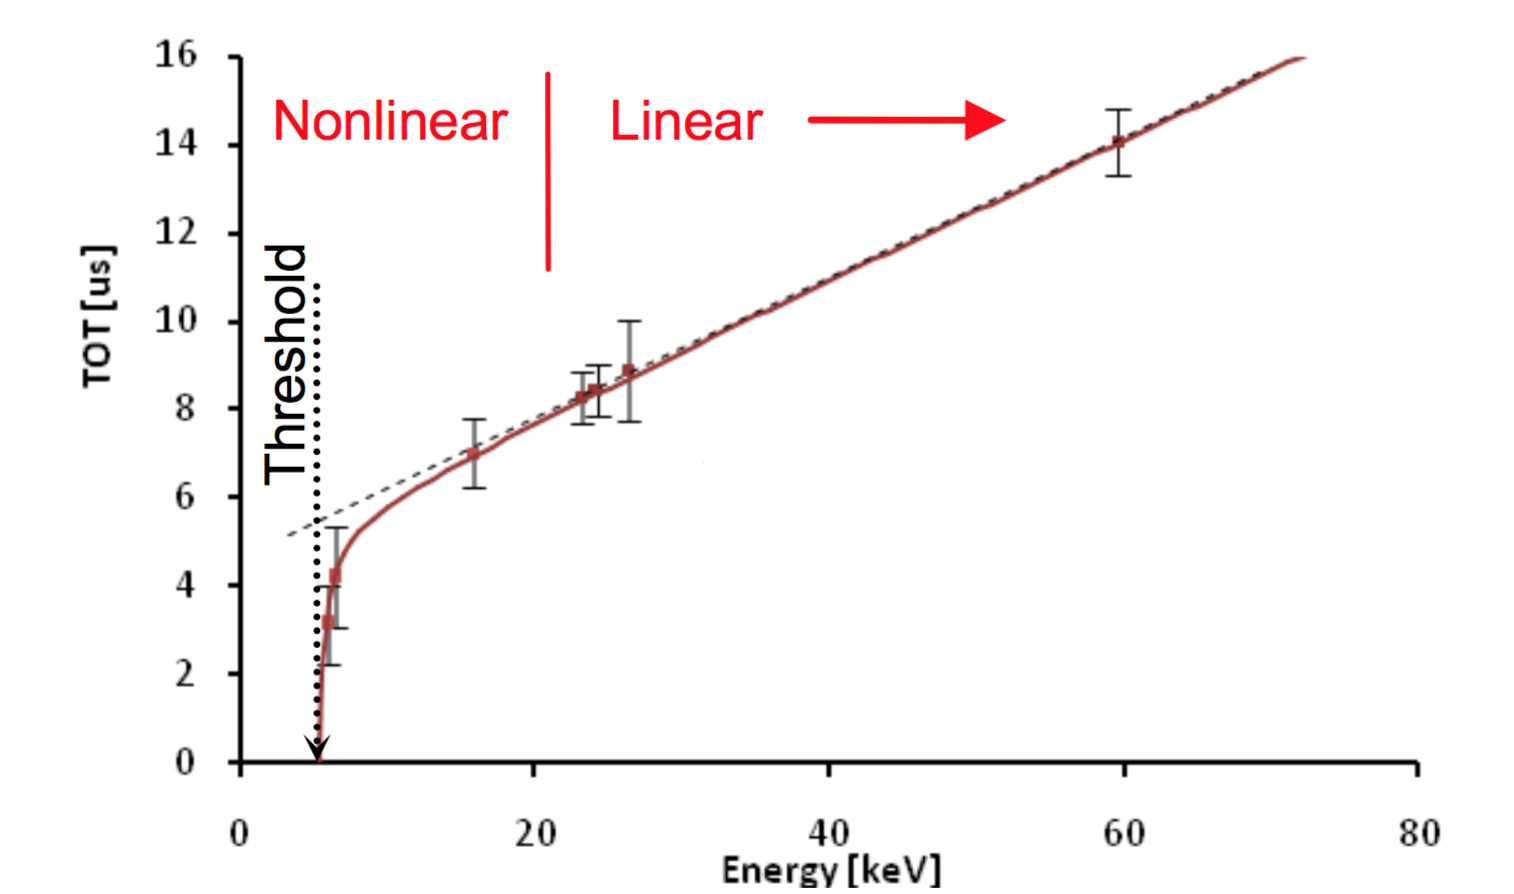
\includegraphics[width=13cm]{figures/calib_function.png}
		\caption{Kalibrační funkce, udávající závislost mezi energií v \texttt{keV} a \texttt{ToT} \cite{Jakubek2011S262}, vzniklá proložením získaných kalibračních bodů funkcí \ref{eq:det:energyCalib} a sestávající se ze dvou částí - (i) nelineární částí pro oblast nižších energií (hyperbola) a (ii) lineární částí pro vyšší energie (přijímka).}
		\label{fig:det:calib:calib_function}
	\end{center}
\end{figure}

V předchozí části práce byl již představen \textit{Time-Over-Treshold} mód (viz \ref{chap:detectors:operation_modes}), ve kterém je detektor schopný měřit deponovanou energii interagovaných v částic, která je udávána v \texttt{ToT}. Jak již bylo ukázáno, vztah mezi energií v \textit{keV} a \texttt{ToT} je nelineární závislost a závisí na fyzikální vlastnostech daného pixelu, což je předmětem energetické kalibrace, která bude v této podkapitole popsána.

Tato metoda \cite{Jakubek2011S262} spočívá v provedení několika sad měření se zdroji ionizujícího záření, jejichž energie jsou předem známy, a v jejich analytickém zpracování a vytvoření kalibrační funkce \ref{eq:det:energyCalib} pro každý pixel detektoru. V předchozí práci \cite{BegeraBcThesis2016} byly tyto metody podrobně popsány a byl vytvořen software, který uživateli umožňuje vytvoření energetické kalibrace detektoru z naměřených dat.

\begin{equation}\label{eq:det:energyCalib}
	f_{calib}(x) = ax + b - \frac{c}{x-t}
\end{equation}

Pro měření kalibračních dat se jako efektivní řešení v praxi ukázalo použití rentgenové fluorescence\footnote{Děj ke kterému dochází při ozařování materiálu (nejčastěji \textit{Cu}, \textit{Fe}, \text{In} apod.) rentgenovým zářením, při kterém jsou z něj vyráženy excitované elektrony. Při vyražení elektronu na nižší energetické úrovni, elektron z vyšší energetické úrovně obsadí jeho místo a přebytečnou energii emituje formou vyzářeného fotonu - fluorescenčního záření, jehož charakteristické monoenergetické spektrum je pro většinu prvků dobře známé.} \cite{Jakubek-radiography_and_charge_sharing}. Pro zajištění dobré kvality kalibrace je třeba naměřit takový počet událostí, aby spektra ve snímcích byla dobře rozeznatelná. Z naměřených dat jsou vyfiltrovány pouze tzv. \textit{Single-hit} události\footnote{Události, ve kterých částice interagovala pouze s jedním pixelem detektoru}, aby se minimalizovaly negativní vlastnosti \textit{Charge-sharing} efektu (díky společné elektrodě senzoru jsou díky interagující částici vzniklé elektrony zpracovány více pixely najednou a část deponované energie nemusí být ASIC čipem zpracována, protože vzniklý signál může být nižší než treshold daného pixelu).

\begin{figure}[th]
	\begin{center}
		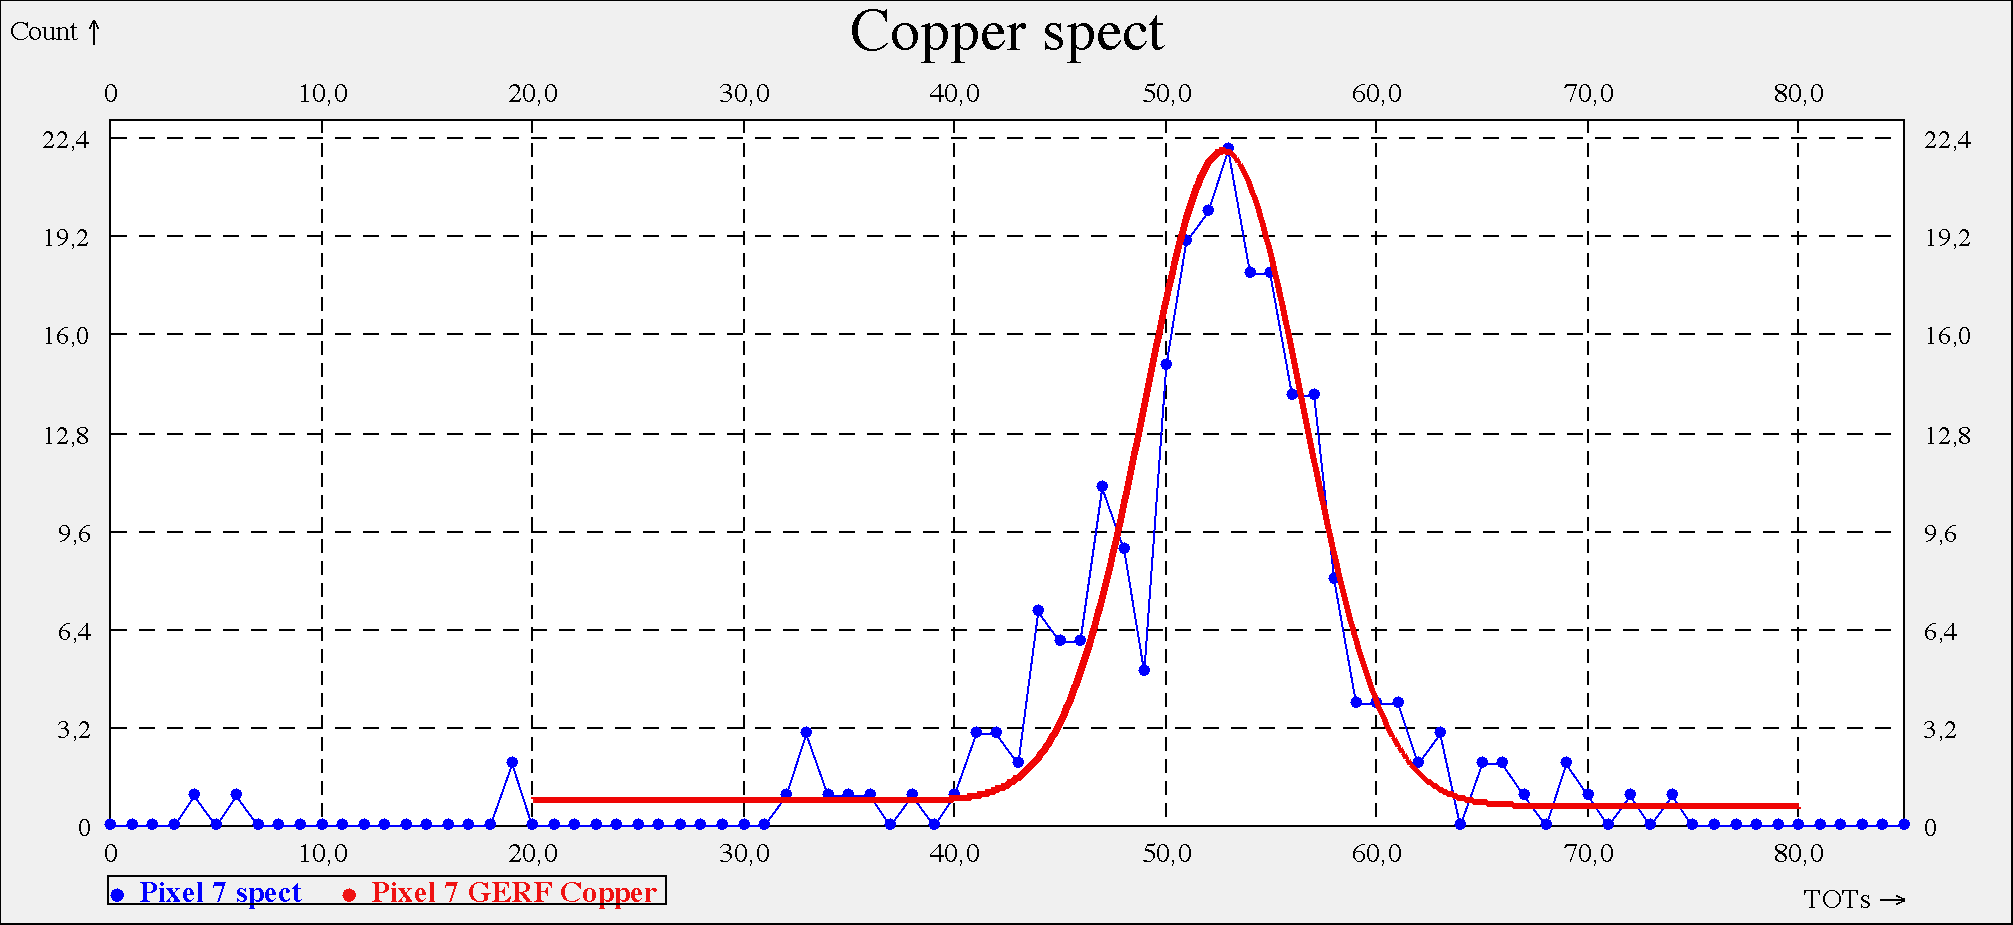
\includegraphics[width=15cm]{figures/calib_gerf.png}
		\caption{Příklad energetického spektra jednoho pixelu Timepix detektoru s proloženou funkcí \ref{eq:det:gerf} \cite{BegeraBcThesis2016}.}
		\label{fig:det:calib:gerf}
	\end{center}
\end{figure}

Z jednotlivých měření jsou pro každý pixel detektoru vytvořena spektra \texttt{ToT} hodnot. Na obrázku \ref{fig:det:calib:gerf} je znázorněn příklad takového spektra, získaného z fluorescence mědi. Požadovaný kalibrační bod se získá střední hodnoty \texttt{ToT} a tabulkové hodnoty energie fluorescenčního záření mědi. Střední hodnota je získána proložením spektra funkcí \ref{eq:det:gerf} - jedná se o součet Gaussovy funkce a Gaussovy chybové funkce (kvůli levé nesymetrii vzniklé \textit{Charge-sharing} efektem)
\begin{equation}\label{eq:det:gerf}
	f_{GERF}(x) = \underbrace{Ae^{ -\frac{(x-\mu)^2}{2\sigma^2} }}_{\text{Gaussova funkce}} +
	\underbrace{ \frac{avg_{right} - avg_{left}}{\sigma\sqrt{2\pi}} \int_{-\infty}^t e^{ -\frac{(t-\mu)^2}{2\sigma^2} } + avg_{left}}_{\text{Gaussova chybová funkce}},
\end{equation}
kde:
\begin{changemargin}{1.5cm}{1cm} 
	\begin{itemize}
		\item [$A$] je amplituda,
		\item [$\mu$] je stření hodnota hledané energie,
		\item [$\sigma$] je rozptyl střední hodnoty energie $\mu$, který je možné vypočítat ze vzorce 
			\ref{eq:det:gerf_sigma}, kde \texttt{FWHM}\footnote{z angl. Full Width at Half Maximum} udává šířku gausiánu v~polovině jeho výšky a
		\item [$avg_{right}$, $avg_{left}$] je průměrná hodnota spektra na pravém (resp. levém) úpatí gausiánu.
	\end{itemize}
\end{changemargin}

\begin{equation}\label{eq:det:gerf_sigma}
	\sigma = \frac{2\sqrt{2ln_2}}{FWHM}
\end{equation}

\subsection{Time-Walk korekce}\label{chap:detectors:calibration:timeWalk}

\textit{Time-Walk} efekt je nežádoucí jev, který vzniká při interakci ionizujícího záření o různé energii. Velikost deponované energie má vliv na amplitudu a sklon napěťového pulzu na zesilovači pixelu. Při interakci ionizující částice s více pixely je pak díky tomuto jevu interagovanými pixely zaznamenána jiná hodnota \textit{Time-of-Arrival} (ToA), i přes to že událost byla způsobena stejnou částicí a ToA by měl být stejný. Viz obrázek \ref{fig:det:calib:timeWalk}, kde jsou pro interakci stejné částice čtyřmi sousedními pixely zaznamenány různé hodnoty ToA. 

\begin{figure}
	\begin{center}
		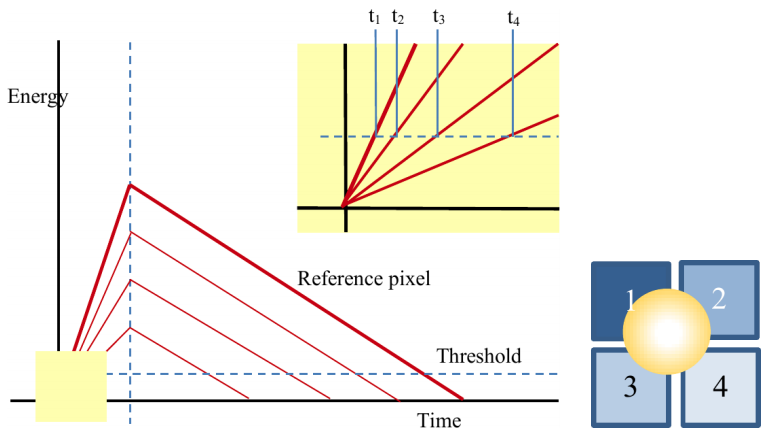
\includegraphics[width=12cm]{figures/calib_timeWalk.png}
		\caption{\textit{Time-walk} efekt: příklad interakce jedné částice se čtyřmi pixely detektoru, kde v každém pixelu byla deponována jiná energie, což na výstupů zesilovačů pixelů způsobilo jiné hodnoty napětí. Díky rozdílné charakteristice náběžné hrany pulzů byl treshold překročen v různých časech ($t_{1-4}$) \cite{Turecek2016TimeWakl}.}
		\label{fig:det:calib:timeWalk}
	\end{center}
\end{figure}

S použitím detektoru \textit{Timepix3}\cite{timepix3} je možné tuto energeticky závislou chybu eliminovat za použití kalibrační metody \cite{Turecek2016TimeWakl}, protože tento detektor umožňuje měřit v ToA a ToT módu současně. Tato kalibrační metoda spočívá v analytickém zpracování dat získaných z měření se zdrojem alfa částic (v \cite{Turecek2016TimeWakl} použito $^{241}$\texttt{Am}), které generuje clustery o velikosti maximálně čtyři pixely. Nejprve je však třeba potřeba energeticky zkalibrovat \ref{chap:detectors:calibration:energy}. 

O vybraných clusterech o velikosti 3 a 4 pixely pro $^{241}$\texttt{Am} víme, že součet jejich energií je $59.5keV$. Z clusteru je vybraný pixel s energií $30keV$, který je použit jako referenční (na \ref{chap:detectors:calibration:timeWalk} jako $t_1$), zbylá energie je náhodně rozdělena mezi ostatní pixely (na \ref{chap:detectors:calibration:timeWalk} jako $t_{2-4}$). Jednotlivé rozdíly $t_i+t_1$ jsou analytickými metodami, popsanými v \cite{Turecek2016TimeWakl}, zpracovány a výsledkem tohoto procesu jsou konstanty $c,d$ pro každý pixel detektoru, kterými lze vypočítat jeho \textit{Time-Walk offset} $\Delta T$:

\begin{equation}\label{eq:det:timeWalk}
	\Delta T = \frac{c}{(E - E_0)^d}
\end{equation}
kde:
\begin{changemargin}{1.5cm}{1cm} 
	\begin{itemize}
		\item [$\Delta T$] je \textit{Time-Walk} korekce pixelu [$ns$] (výsledná hodnota ToA je pak rovna $ToA-\Delta T$),
		\item [$E$] je energie pixelu [keV],
		\item [$E_0$] je treshold pixelu [keV] a
		\item [$c,d$] jsou konstanty.
	\end{itemize}
\end{changemargin}

\subsection{ToA offset korekce}\label{chap:detectors:calibration:toa_correction}
Jedná se o jev, ke kterému dochází u \textit{Timepix3} detektorů z důvodu chyby hardware, který způsobuje špatnou synchronizaci časového razítka napříč sloupci detektoru \cite{Katherine}. Tato chyba vzniká jen při zapnutí detektoru a poté je \texttt{ToA} offset již stabilní, takže je možné vytvořit korekci.

Odstranění tohoto jevu spočívá ve vytvoření kompenzační tabulku pomocí středních hodnot interních testovacích pulzů \cite{timepix3}. Pro získání správných hodnot \texttt{ToA} z naměřených dat stačí jen odečíst příslušnou hodnotu z korekční tabulky.

%********************************************************************************
% Přehled detektorů rodiny Medipix
%********************************************************************************
\section{Přehled detektorů rodiny Medipix}\label{chap:detectors:medipix_overview}
V této podkapitole budou stručně představeny jednotlivé detektory, které byly vyvinuty v rámci Medipix kolaborace \cite{medipix-www}.

\begin{figure}
	\begin{center}
		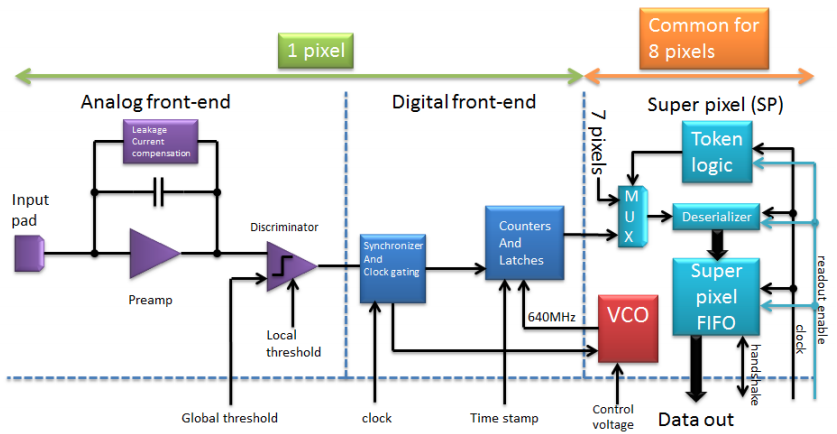
\includegraphics[width=15cm]{figures/det_timepix3_schema.png}
		\caption{Schéma pixelu detektoru \textit{Timepix3} se společnou elektronikou pro 8 pixelů (tzv.\textit{Super-pixel}) \cite{timepix3}.}
		\label{fig:det:medipix_overview:timepix3_schema}
	\end{center}
\end{figure}

\begin{description}

	\item[Medipix1] V roce 1998 byl vyvinut detektor \textit{Medipix1} \cite{medipix1}, také zvaný \textit{Photon-Counting-Chip}, byl první velkoplošný detektor používající CMOS technologie. S maticí $64\times64$ pixelů, každým o hraně $170~\mu m$, má celkovou aktivní plochu $1,1~cm^2$. I přes malý počet pixelů a jejich velkou rozteč, tento detektor prokázal dobré rozlišovací vlastnosti, především pak v rentgenovém zobrazování. 
	
	Detektor je vyrobený pomocí $1~\mu m$ technologie a je schopný operovat pouze v Medipix módu (viz \ref{fig:det:modes}) a podporuje pouze vyčítání po snímcích (viz \ref{chap:detectors:readout}).
	
	\item[Medipix2] V roce 2001 byl vyvinut detektor \textit{Medipix2} \cite{medipix2}, jako náhrada za svého předchůdce \textit{Medipix1}. Díky $250~nm$ technologii bylo možné zvýšit počet pixelů a zároveň snížit jejich rozteč - detektor má $256\times256$ pixelů, každý o hraně $55~\mu m$. Navíc má dva tresholdy s diskriminací na 4 pixely. 
	
	Stejně jako svůj předchůdce je schopný operovat pouze v Medipix módu (viz \ref{fig:det:modes}) a podporuje pouze vyčítání po snímcích (viz \ref{chap:detectors:readout}).
	
	\item[Timepix]\label{chap:detectors:medipix_overview:timepix} V roce 2006 byl vyvinut detektor \textit{Timepix} \cite{timepix}, který vychází z detektoru \textit{Medipix2}. Detektory mají stejné rozměry, ale architektura pixelů se změnila. Nově každý pixel detektoru umožňuje nezávisle měřit čas interakce částice, její energii, nebo je schopný počítat jednotlivé interakce. 
	
	Detektor je schopný operovat v \texttt{ToT}, \texttt{ToA}, nebo v Medipix módu (viz \ref{fig:det:modes}) a podporuje pouze vyčítání po snímcích (viz \ref{chap:detectors:readout}).
	
	\item[Medipix3] V roce 2011 byl vyvinut detektor \textit{Medipix3} \cite{medipix3}, jako nástupce \textit{Medipix2} detektoru. Rozměry detektoru zůstaly zachovány ($256\times256$ pixelů, každý o hraně $55~\mu m$), ale díky $130~nm$ technologii byla funkce jednotlivých pixelů vylepšena. Detektor nově umožňuje zvýšení energetického rozlišení díky potlačení \textit{Charge-Sharing} efektu (viz \ref{chap:detectors:calibration:energy}) pomocí integraci náboje do clusteru $4\times4$ pixelů. 
	
	Každý pixel má dva 14-bitové čítače. Jednotlivé pixely můžou být naprogramovány tak, aby vždy měřily za pomocí jednoho čítače, zatímco je hodnota z druhého čítače vyčítána, což umožňuje měření bez mrtvé doby.

	Také je možné zapojit tento readout čip (s pixelem o hraně $55~\mu m$) na senzor s pixely o hraně $110~\mu m$, takže výsledný super-pixel má k dispozici 8 čítačů a pomocí různých úrovní tresholdů jej lze použít jako 8-kanálový spektrometr.

	Stejně jako svůj předchůdce je schopný operovat pouze v Medipix módu (viz \ref{fig:det:modes}) a podporuje pouze vyčítání po snímcích (viz \ref{chap:detectors:readout}).

	\item[Timepix3]\label{chap:detectors:medipix_overview:timepix3} V roce 2014 byl vyvinut detektor \textit{Timepix3} \cite{timepix3}, jako nástupce \textit{Timepix} detektoru. Rozměry byly zachovány, ale bylo použita $130~\mu m$ výrobní technologie, jako u \textit{Medipix3}. Detektor nově umožňuje měřit v \texttt{ToA} a \texttt{ToT} současně a jeho časové rozlišení bylo vylepšeno více než na šestinásobek.

	Detektor nově umožňuje kromě vyčítání po snímcích i \textit{Data-Driven} mód, kde jsou data v rámci akvizice kontinuálně z detektoru vyčítána (viz \ref{chap:detectors:readout}). Takto navržená architektura umožňuje vyčítat data až do $40M_{hits}*cm^{-2}*s^{-1}$ bez globální mrtvé doby detektoru (pouze s lokální mrtvou dobou - pro jednotlivé pixely, ze kterých jsou vyčítána naměřená data).

	Na obrázku \ref{fig:det:medipix_overview:timepix3_schema} je znázorněno blokové schéma jednoho pixelu \textit{Timepix3} detektoru, který se skládá z analogové a digitální části (pro popis funkcionality viz \ref{chap:detectors:princip}). Na obrázku vpravo je pak společná elektronika, sdílená vždy 8 sousedními pixely (tzv.\textit{Super-pixel}).

\end{description}

%********************************************************************************
% Vyčítací rozhraní
%********************************************************************************
\section{Vyčítací rozhraní}\label{chap:detectors:readouts}
V této podkapitole bude popsáno několik vyčítacích rozhraní, které byly vyvinuty (v rámci \textit{Medipix kolaborace}\footnoteUrl{https://medipix.web.cern.ch}) ÚTEF ČVUT v Praze a jeho spinoff společností ADVACAM s.r.o. Pro komunikaci s \textit{Timepix3} detektorem bude v rámci této práce bude použito nově vyvinuté vyčítací rozhraní \textbf{Katherine} \cite{Katherine} \ref{chap:detectors:readouts:katherine}.

\subsection{FITPix}
FITPix \cite{fitpix} vyčítací rozhraní bylo vyvinuto v roce 2010 a skládá ze z programovatelného hradlového pole (\texttt{FPGA})\footnote{Z angl. Field Programmable Gate Array}, USB 2.0 rozhraní, DAC\footnote{Převodník digitálního signálu na analogový.} a ADC\footnote{Převodník analogového signálu na digitální.} převodníků a obvodů pro generování měřícího napětí (\textit{bias}).

Zařízení je s detektorem propojeno pomocí \textit{LVDS}\footnote{Z angl. Low-voltage differential signaling} a je schopné jeho plnohodnotného řízení, vč. nastavování hodnot (měřící frekvence, treshold, bias apod.), řízení akvizice a vyčítání naměřených dat rychlostí až $90$ snímků za sekundu. Zařízení rovněž umožňuje připojení externího trigger signálů pro synchronizované měření s více detektory současně.

FITPix je možné použít pouze jako nízkoúrovňové vyčítací rozhraní a veškerá business logika musí být implementována v připojeném počítači (na př. deserializace a derandomizace naměřených dat apod.). Jako řídící software je použit \textit{Pixelman}\cite{pixelman}. Zařízení je kompatibilní se všemi detektory uvedenými v \ref{chap:detectors:medipix_overview}, kromě \textit{Timepix3}.

\subsection{AdvaDAQ}
AdvaDAQ \cite{Turecek2016TimeWakl} je nástupcem vyčítacího rozhraní FITPix a kompatibilní se všemi detektory uvedenými v \ref{chap:detectors:medipix_overview}. Principem funkce vychází ze svého předchůdce, ale díky použitému rozhraní USB 3.0 je schopné dosahovat maximálního datového toku $2,9~Gb/s$. Deserializace naměřených dat byla implementována do firmware \textit{FPGA}. Pro řízení tohoto rozhraní, vizualizaci a analýzu naměřených dat byl vyvinut software Pixet.

\subsection{ATLAS Pix}\label{chap:detectors:readouts:atlaspix}
ATLAS Pix \cite{atlastpx_sw, BegeraBcThesis2016} je zařízení vyvinuté v rámci experimentu \textit{ATLAS-TPX}, síti 16 hybridních částicových detektorů \textit{Timepix}, instalované v rámci experimentu \textit{ATLAS} na \textit{LHC} v \textit{CERN}, operující od roku 2014.

Zařízení vzniklo modifikací vyčítacího rozhraní \textit{FITPix} a disponuje \texttt{FPGA}, \texttt{LVDS} zesilovačem a počítače \textit{Raspberry Pi}, ve kterém je implementován software, poskytující API pro své vzdálené řízení přes \texttt{TPC} protokol. Komunikace mezi \texttt{FPGA} a počítačem je realizována pomocí \texttt{SPI}\footnote{Z angl. Serial Peripheral Interface.} protokolu.

\subsection{Katherine}\label{chap:detectors:readouts:katherine}
\begin{figure}
	\begin{center}
		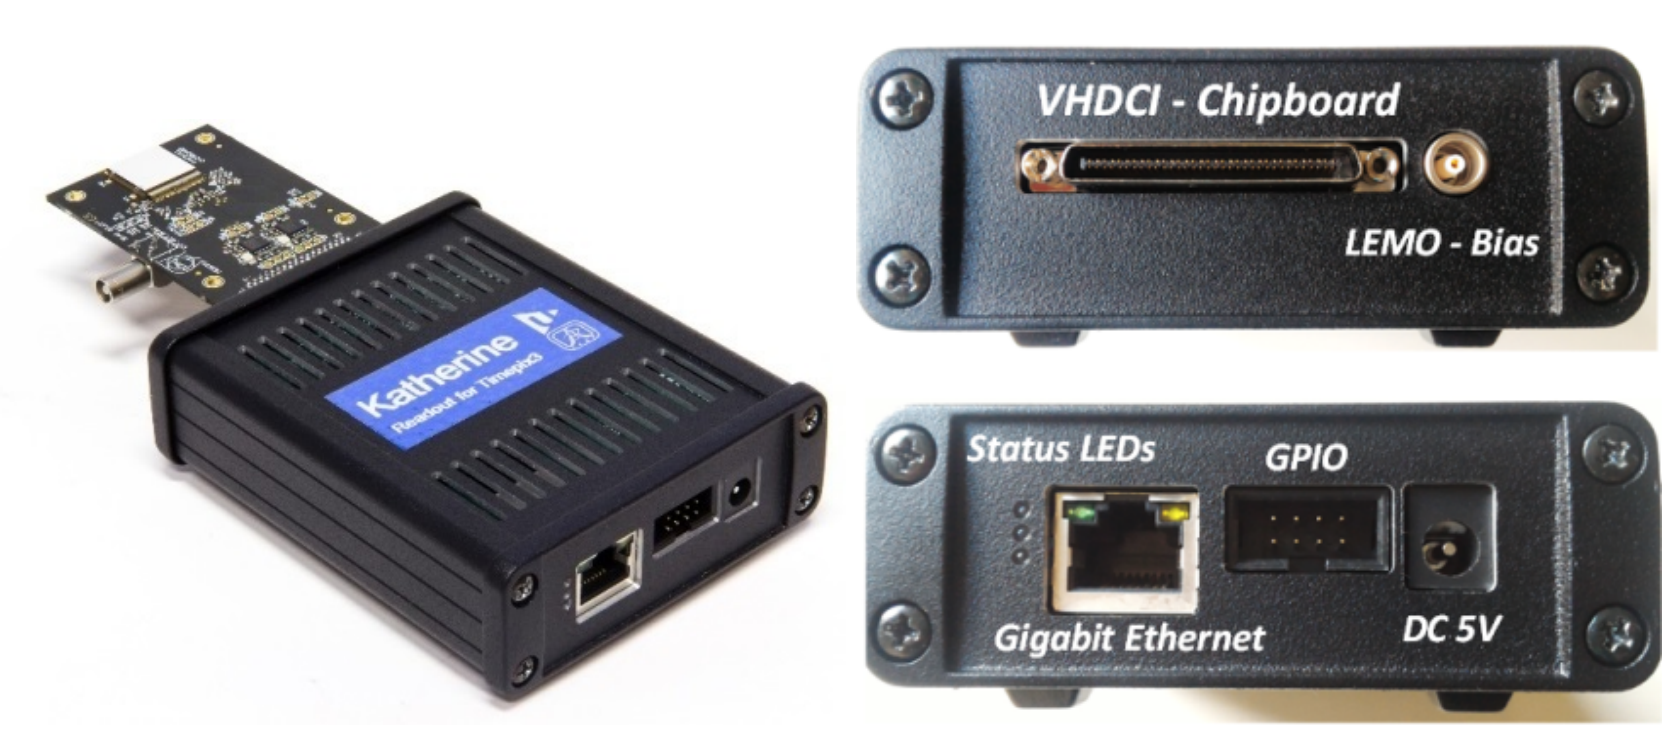
\includegraphics[width=15cm]{figures/det_katherine.png}
		\caption{Vyčítací rozhraní \textit{Katherine} s přípojeným detektorem \textit{Timepix3} vlevo a popisem vstupných a výstupních portů vpravo\cite{Katherine}.}
		\label{fig:det:readout:katherine}
	\end{center}
\end{figure}

Katherine \cite{Katherine} je pokročilé vyčítací rozhraní dedikované pro řízení jednoho \textit{Timepix3} detektoru, které v sobě obsahuje embedovaný počítač, čímž se vymezuje od ostatních vyčítacích rozhraní bez procesoru, kde business logika musí být implementována v připojeném počítači, což má negativní dopad na vytížení jeho procesoru. 

Hlavním benefitem zařízení je možnost jeho použití na experimentech, kde je nutná větší vzdálenost mezi detektorem a vyčítacím rozhraním (u \textit{Katherine až $100~m$}). Toto omezení je dáno především nedostatečnou radiační a elektromagnetickou odolností použité elektroniky. To umožňuje aplikace v blízkosti jaderných reaktorů nebo na částicových urychlovačích (na příklad měření luminosity v rámci experimentu ATLAS na LHC v CERN \cite{atlastpx_luminosity}). 

Zařízení je kompatibilní s \textit{Timepix3} detektory, které jsou osazeny na CERN chipboard, nebo na kompatibilní \texttt{PCB}\footnote{Z angl. Printed Circuit Board.} s \texttt{VHDCI}\footnote{Z angl. Very-High-Density-Cable-Interconnect.} 68-pinovým konektorem. S detektorem může být propojeno na přímo (viz obr. \ref{fig:det:readout:katherine} vlevo), prodlužovacím \texttt{VHDCI} kabelem o maximální délce až $10~m$, nebo speciálním extenderem na bázi ethernetu pro vzdálenosti až $120~m$. S rostoucí vzdáleností ale klesá maximální datový tok (viz tabulka \ref{tab:det:katherine:data_flow}).

\begin{table}[th]
	\begin{center}
		\begin{tabular}{|c|c|c|c|}
			\hline
			\textbf{Vzdálenost} & \textbf{Typ propojení} & \textbf{Počet kanálů - datový tok} & \textbf{Hit Rate} \\
			\hline
			$3~m$ & VHDCI & $2 \times 640~Mb/s$ & $16~M_{hits}/s$\\
			$10~m$ & VHDCI & $4 \times 160~Mb/s$ & $10~M_{hits}/s$\\
			$20~m$ & Ethernet & $2 \times 640~Mb/s$ & $16~M_{hits}/s$\\
			$100~m$ & Ethernet & $4 \times 80~Mb/s$ & $5~M_{hits}/s$\\
			\hline
		\end{tabular}
	\end{center}
	\caption{Katherine: závislost maximálního datového toku na typu propojení mezi detektorem a vyčítacím rozhraním \cite{Katherine}.}
	\label{tab:det:katherine:data_flow}
\end{table}

Jeho maximální výstupní datový tok je daný použitým gigabitovým ethernetem, které odpovídá ekvivalentu datového toku $16M_{hits}*cm^{-2}*s^{-1}$ v \textit{Data-Driven} módu (viz \ref{chap:detectors:readout}). \textit{Timepix3} detektor je schopný generovat až $80M_{hits}*cm^{-2}*s^{-1}$, takže při vyšší zátěži není zařízení schopné přenést všechny zaznamenané události. Nicméně, \textit{Katherine} disponuje vestavěnou \texttt{DDR3} pamětí o velikosti $1~GB$, která funguje jako buffer - když je aktuální počet zpracovávaných událostí vyšší, než je maximální datový tok spojení s nadřazeným počítačem, tak se data hromadí v bufferu, aby později při nižší intenzitě zpracovávaných událostí mohly být přeneseny.

Pro úplnost výčtu vstupních a výstupných portů je třeba doplnit, že \textit{Katherine} také disponuje \texttt{GPIO}\footnote{Z angl. General Purpose Input/Output.} konektorem (viz obr. \ref{fig:det:readout:katherine} vpravo), zahrnující 4 obecné signály pro integraci s dalšími zařízeními a další rozšíření, jako na příklad pro trigger synchronizaci (pro možnost zapojení na příklad do detektorového teleskopu \cite{katherine_telescope}). Zařízení dále disponuje \texttt{LEMO} konektorem (viz \ref{fig:det:readout:katherine}), poskytujícím vysokonapěťový zdroj ($\pm300~V$) pro \textit{bias} (měřící napětí) detektoru.

Vyčítací rozhraní má implementovanou podporu pro \texttt{ToA} korekci (viz \ref{chap:detectors:calibration:toa_correction}), které je automaticky vykonána v rámci startovací sekvence, kde jsou poškozené sloupce identifikovány pomocí středních hodnot testovacích pulzů a je sestavena kompenzační tabulka. V průběhu akvizice dat jsou \texttt{ToA} hodnoty automaticky opraveny odečtením příslušných hodnot z výše zmíněné tabulky.

\subsubsection{Komunikace s nadřazeným PC a řízení akvizice dat}
Vyčítací rozhraní \textit{Katherine} je dle dané konfigurace schopné operovat ve dvou módech:

\begin{description}
	\item [SFTP klient (autonomní mód)] V tomto módu zařízení operuje z pohledu řízení a akvizice dat zcela nezávisle. Po spuštění zařízení, resp. dokončení startovací sekvence, jsou z dodané konfigurace automaticky nastaveny měřící a akviziční parametry detektoru a je spuštěna akvizice dat. Získaná data jsou pak nepřetržitě posílána pomocí \textit{SFTP}\footnote{Z angl. Secure File Transfer Protocol (protokol pro zabezpečený přenos souborů mezi počítači pomocí \texttt{TPC} protokolu).} na server, kde jsou data ukládána do definovaného adresáře v \texttt{ASCII} souborech. Výhoda tohoto módu spočívá v jednoduchosti obsluhy a hodí se především pro takové aplikace, kde není očekáván vysoký datový tok a kde není potřeba měnit nastavení detektoru, protože každé jeho změna vyžaduje restart zařízení.
	
	\item [Manuální mód] Pracuje-li zařízení v tomto módu, pak k jeho funkci je třeba řízení z nadřazeného počítače pomocí proprietárního \texttt{UDP}\footnote{Z angl. User Datagram Protocol.} protokolu. Protokol využívá dvou \texttt{UDP} portů - \textbf{řídícího} a \textbf{datového}.

	\begin{description}
		\item [Komunikační] port je vyhrazen pro pro přenos řídících a konfiguračních paketů. Komunikace je implementována pomocí $36$ příkazů, kde každý z nich se skládá 64-bitového datagramu pro request a 64-bitového datagramu pro response, takže se jedná o synchronní potvrzovanou komunikaci\footnote{Potvrzování je realizováno na aplikační úrovni \texttt{ISO/OSI} modelu.}. Pro příklad viz obrázek \ref{tab:det:katherine:comm:packet_example}, kde je zobrazen request datagramu pro vyčtení biasu a jeho response.
		
		\item [Datový] port je určen pro jednosměrnou komunikaci z \textit{katherine} do nadřazeného počítače a slouží k přenosu naměřených dat. každý datagram se skládá z 3-bitové hlavičky 43-bitových dat.
	\end{description}
	
\end{description}

\begin{figure}[]
	\begin{center}
		\begin{bytefield}[endianness=big,bitwidth=0.52em]{64}
			\begin{rightwordgroup}{Odchozí\\datagram}
				\bitheader{63,56,48,40,32,24,16,8,0} \\
				\bitbox{16}{\textbf{Command ID}} & \bitbox{48}{\textbf{Command data}} \\
				\bitbox{16}{0x0C} & \bitbox{8}{-} & \bitbox{8}{bias id} & \bitbox{32}{-}
			\end{rightwordgroup}
		\end{bytefield}
		
		\begin{bytefield}[endianness=big,bitwidth=0.52em]{64}
			\\ \\ \\
			\begin{rightwordgroup}{Příchozí\\datagram}
				\bitheader{63,56,48,40,32,24,16,8,0} \\
				\bitbox{16}{\textbf{Command ID}} & \bitbox{48}{\textbf{Command data}} \\
				\bitbox{16}{0x0C} & \bitbox{16}{-} & \bitbox{32}{bias (float)}
			\end{rightwordgroup}
		\end{bytefield}
	\end{center}
	\caption{Katherine: příklad requestu a response řídícího datagramu pro vyčtení biasu.}
	\label{tab:det:katherine:comm:packet_example}
\end{figure}

V rámci této práce bude použit druhý zmíněný - manuální mód, protože je méně náročný na šířku pásma a umožňuje vzdálené řízení detektoru. V dalších kapitolách (viz \todo ref) bude komunikační rozhraní vyčítacího rozhraní \textit{Katherine} popsáno podrobněji.
\addbibresource{reference.bib}

\chapter{Návrh architektury}\label{chap:arch}
V této kapitole bude čtenář seznámen s návrhem a koncepcí softwarového systému \textbf{Pixnet} -- software pro distribuované řízení sítě částicových pixelových detektorů, který byl navržen a implementován v rámci této práce. V této kapitole bude popsána motivace pro vznik tohoto systému a budou představeny jednotlivé komponenty systému a jejich vzájemná komunikace. Pro detailnější popis návrhu a implementace komponent viz kapitoly \ref{chap:handler}, \ref{chap:katherine} a \ref{chap:master}.

%********************************************************************************
% Motivace
%********************************************************************************
\section{Motivace}\label{chap:arch:motivation}
Hlavní motivací pro vznik tohoto systému je fakt, že moderní částicové pixelové detektory jsou schopné generovat velký datový tok, například \textit{Timepix3} má teoretické maximum \unit{5,12}{Gb/s} (viz \ref{chap:detectors:medipix_overview:timepix3}), takže nedistribuovaný systém, který by operoval na jedné instanci, by nebyl schopný zpracovat datový tok, který je síť o více detektorech schopna generovat. 

Zde je možné namítnout, že každý systém je možné škálovat vertikálně\footnote{Škálováním v kontextu počítačových systémů rozumíme změnu vlastností daného systému za účelem zvýšení, nebo snížení jeho výpočetního výkonu (ev. jiného sledovaného parametru). Zatímco u vertikálního škálování měníme vlastnosti jednoho uzlu systému (například přidáváním procesorů, pamětí, kapacity úložiště apod.), u horizontálního škálování přidáváme jednotlivé uzly -- samostatné  jednotky (např. počítače). Pro úplnost je třeba doplnit, že vertikální škálování má své omezení z hlediska použitého hardware, u horizontálního škálování žádná taková omezení nejsou.}. Zatímco cenu škálování horizontálně škálovatelného systému zle popsat lineární závislostí výpočetního výkonu na ceně, u vertikálně škálovatelného systému tato závislost roste exponenciálně. Jelikož vertikální škálování takového systému je  vysoce neefektivní, nebude dále uvažováno a tato práce se bude věnovat jenom návrhu a implementaci horizontálně škálovatelného řešení.

 Další motivací pro vytvoření tohoto systému je možnost řízení heterogenní sítě detektorů homogenním způsobem. Heterogenní sítí detektorů rozumíme takovou síť, ve které jsou detektory různých typů (například \textit{Timepix}, \textit{Timepix3} apod, viz \ref{chap:detectors:medipix_overview}), komunikující různými komunikačními protokoly prostřednictvím různých vyčítacích rozhraních (například \textit{Katherine}, \textit{ATLAS Pix} apod, viz \ref{chap:detectors:readouts}). V další části textu bude detailně popsána navržená a implementovaná modulová architektura, která výše zmíněné umožňuje.

 Pro potřeby experimentu \textit{ATLAS-TPX} byl již vyvinut software \cite{atlastpx_sw,BegeraBcThesis2016} pro řízení sítě detektorů \textit{Timepix} \ref{chap:detectors:medipix_overview:timepix}, prostřednictvím vyčítacího rozhraní \textit{ATLAS Pix} \ref{chap:detectors:readouts:atlaspix}. Software však nevyhovuje požadavkům diskutovaných výše:
 \begin{enumerate}[label=(\roman*)]
     \item \textbf{Škálovatelnost} -- systém je navržen bez možnosti horizontálního škálování. Všechny detektory sítě jsou řízeny z jednoho uzlu a všechna vygenerovaná data jsou jím zpracovávána. Možnost použití pouze jednoho uzlu představuje nejslabší článek systému, který nemůže být použit pro řízení a vyčítání dat z větší sítě detektorů.
     \item \textbf{Modularita} -- systém implementuje pouze komunikační protokol vyčítacího rozhraní \textit{ATLAS Pix} \ref{chap:detectors:readouts:atlaspix}. Přidání podpory nového vyčítacího rozhraní představuje významnou modifikaci architektury systému a pro nasazení nové verze je nutná odstávka celého systému.
 \end{enumerate}
Pro potřeby modernizace sítě \textit{ATLAS-TPX} (za použití detektorů \textit{Timepix3}) bylo rozhodnuto o vývoji software, který bude navržen a implementován tak, aby požadavky na škálovatelnost a modularitu byly zohledněny.

%********************************************************************************
% Softwarová architektura
%********************************************************************************
\section{Softwarová architektura}\label{chap:arch:sw}
V této podkapitole budou popsány jednotlivé komponenty softwarové architektury systému Pixnet a bude vysvětlena jejich funkce. Na obrázku \ref{fig:arch:sw_architecture} jsou zobrazeny základní komponenty systému, včetně jejich kardinalit. Detektory sítě jsou řízeny handlery, které komunikují s detektory pomocí dodaného komunikačního protokolu (na obr. \ref{chap:arch:sw} jako \textit{komunikační interface}) a vyčítají z nich data, která jsou pak ukládána do datového úložiště (pomocí dodané implementace datového interface). Jednotlivé handlery jsou řízeny centrálním uzlem systému -- masterem. Master je zodpovědný za konfiguraci systému, držení jeho stavu a přiřazování detektorů masterům.

\begin{figure}[h]
	\begin{center}
		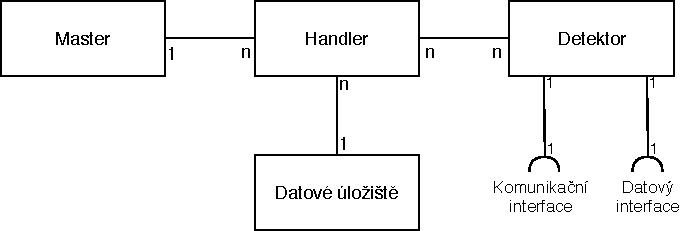
\includegraphics[width=14.5cm]{figures/arch_sw.pdf}
		\caption{Pixnet: softwarová architektura.}
		\label{fig:arch:sw_architecture}
	\end{center}
\end{figure}

V následujících podkapitolách budou detailněji popsány jednotlivé komponenty z obrázku~\ref{chap:arch:sw}.
\subsection{Detektor}\label{chap:arch:sw:detector}
Detektor je logická jednotka systému, která je reprezentována implementací komunikačního a datového interface, konfigurací a svým stavem. Fyzické propojení s detektorem je realizováno implementací komunikačního interface.

Komunikační interface obsahuje například metody pro navazování spojení s detektorem, metody pro nahrávání konfigurace a metody pro získání podporovaných příkazů detektoru a jejich vykonání. Každý příkaz má svoje ID, název a model vstupních a výstupních hodnot. Modelem hodnot rozumíme množinu parametrů různých datových typů (\texttt{boolean}, \texttt{integer}, \texttt{float} apod.), které mohou nabývat hodnot omezených zadaným intervalem, nebo jedné z předdefinovaných diskrétních hodnot.

Datový interface obsahuje kromě inicializačních metod (předání konfigurace detektoru apod.) také metodu pro předání reference na asynchronní frontu naměřených dat, do které jsou data vkládána implementací komunikačního interface. Datový interface může mít několik implementací -- například data mohou být ukládána do datového úložiště handleru a následně asynchronně nahrána do centrálního datového úložiště, nebo mohou být rovnou synchronně nahrávána do datového úložiště.

\subsection{Datové úložiště}
Klíčový požadavek na datové úložiště je škálovatelnost, jelikož pro sítě o vetším počtu detektorů by ukládání dat do jednoho uzlu znamenalo omezení maximálního datového toku, dané kapacitou daného uzlu.

Jednou z možností implementace může být využití distribuovaného souborového systému, například \textit{Hadoop Distributed File System} \cite{HDFS}, který se v praxi\footnote{například v roce 2010 internetová společnost \textit{Yahoo!} používala \texttt{HDFS} pro persistenci \unit{25}{PB} podnikových dat \cite{HDFS}.} používá pro distribuované ukládání dat s možností jejich redundance na více uzlech (pro potřeby zálohování). 

Další možností může být použití některé z \texttt{NoSQL} distribuovaných databází, například \textit{MongoDB} (viz \ref{chap:arch:technologie:mongodb}).

\subsection{Handler}
Handler je komponenta, kterou je řízena podmnožina detektorů detektorové sítě. K jednomu handleru je tedy možné připojit $n$ detektorů, kde $n$ je omezeno sumou datového toku přes všechny připojené detektory v závislosti na maximálním možném datovém toku handleru.

Handler komunikuje s detektorem pomocí dodané implementace jeho komunikačního interface a data detektorem vygenerovaná jsou pomocí implementace datového interface uložena do datového úložiště, nebo zpracována jiným způsobem.

Handler je zodpovědný za zavedení dodaných implementací komunikačního a datového interface do systému. Například po přiřazení detektoru handleru, handler získá seznam podporovaných příkazů detektoru a poskytne je masteru. To systému umožňuje řízení heterogenní sítě detektorů homogenním způsobem, jak již bylo zmíněno v \ref{chap:arch:motivation}.

Aby bylo možné handlery, potažmo detektory, řídit centralizovaně, handler poskytuje \texttt{API}\footnote{Z angl. \textit{Application programming interface} (aplikační programové rozhraní).}. Pomocí \texttt{API} jsou jednotlivé handlery připojovány do systému, handlerům jsou přiřazovány a odebírány detektory, inicializuje se konfigurace detektorů a je řízena akvizice dat.

\subsection{Master}
Master je centrální prvek systému, jehož prostřednictvím jsou řízeny handlery. Master poskytuje \texttt{API} pro své řízení pomocí pomocí frontendové aplikace. Tato aplikace je webový tenký klient, který uživateli poskytuje uživatelské rozhraní pro řízení systému.

Když uživatel přidává nový detektor do systému, tak nejprve skrze uživatelské rozhraní frontend aplikace zadá parametry detektoru, včetně implementace komunikačního a datového rozhraní, jak je znázorněno na obr. \ref{fig:arch:handler:new_detector}. Poté je detektor nahrán do mastera pomocí jeho \texttt{API}, kde je následně perzistentně uložen do jeho databáze. Při přiřazování detektoru handleru je konfigurace detektoru včetně implementace komunikačního a datového interface nahrána do zvoleného handleru, kde je dále zpracována. Zpracování konfigurace probíhá v následujících krocích:
\begin{enumerate}
    \item Vytvoření instance komunikačního interface a ověření jeho validity.
    \item Vytvoření instance datového interface a ověření jeho validity.
    \item Syntaktická analýza (tzv. \textit{parsing}) konfigurace detektoru a její nahrání do instancí komunikačního a datového interface.
    \item Vytvoření asynchronní fronty měřených dat a její předání instancím komunikačního a datového interface.
\end{enumerate}
Po dokončení inicializační sekvence je uživatel notifikován a v případě úspěšného dokončení je detektor připraven vykonávat příchozí příkazy a měřit data.

\begin{figure}[th!]
	\begin{center}
		\begin{sequencediagram}
            \newthread[blue_ligh]{mf}{Master frontend}
            \newinst[0.5]{mb}{Master backend}
            \newinst[0.5]{h}{Handler}
            \newinst[0.5]{d}{Detektor}
            \newinst[0.19]{c}{\shortstack{Impl kom.\\interface}}
            \newinst[0.19]{p}{\shortstack{Impl dat.\\interface}}
            
            % nahrání konfigurace
            \postlevel
            \begin{call}{mf}{
                %pro úpravu thread color
                %\tikzset{threadstyle/.style={top color=white,bottom color=red}}
                    \shortstack{
                        Přidání nového\\
                        detektoru
                    }
                }{mb}{výsledek}
                
                \begin{callself}{mb}{\shortstack{Validace a uložení\\konfigurace detektoru}}{výsledek}
                    \postlevel
                \end{callself}	
                
            \end{call}

            % binding
            \postlevel
            \postlevel
            \begin{call}{mf}{\shortstack{Přiřazení detektoru\\handleru}}{mb}{výsledek}
                
                \postlevel
                \begin{call}{mb}{\shortstack{Přiřazení\\detektoru}}{h}{výsledek}
                    
                    \begin{call}{h}{\shortstack{Inicializace}}{d}{výsledek}
                        
                        \begin{call}{d}{\shortstack{Inicializace\\(konfig.,\\fronta dat)}}{c}{}
                        \end{call}
                        
                        \postlevel
                        \postlevel
                        \begin{call}{d}{\shortstack{Inicializace\\(konfig., fronta dat)}}{p}{}
                        \end{call}

                        %\begin{call}{d}{\shortstack{Zavedení\\modulu}}{c}{}
                        %\end{call}
    
                        %\begin{call}{d}{\shortstack{Zavedení modulu}}{p}{}
                        %\end{call}

                        %\postlevel
                        %\begin{call}{d}{\shortstack{Nahrání\\konfigurace}}{c}{}
                        %\end{call}

                        %\begin{call}{d}{\shortstack{Nahrání konfigurace}}{p}{}
                        %\end{call}
        
                        %\begin{messcall}{d}{\shortstack{Fronta dat}}{c}
                        %\end{messcall}

                        %\begin{messcall}{d}{\shortstack{Fronta dat}}{p}
                        %\end{messcall}
        
                    \end{call}
        
                \end{call}

            \end{call}
            
		\end{sequencediagram}
		\caption{Sekvenční diagram znázorňující příklad přidání detektoru do systému a jeho přiřazení handleru.}
		\label{fig:arch:handler:new_detector}
	\end{center}
\end{figure}

Jako datové úložiště pro konfigurace detektorů, informace o jejich stavu a o stavu jednotlivých handlerů bude navržena relační \texttt{SQL}\footnote{Z angl. \textit{Structured Query Language} (strukturovaný dotazovací jazyk).} databáze, ke které bude přistupovat pouze backend mastera.

%********************************************************************************
% Hardwarová architektura
%********************************************************************************
\section{Hardwarová architektura}\label{chap:arch:hw}
V předchozí podkapitole byla popsána softwarová architektura. Fyzická instalace sítě přináší další omezení, především z pohledu síťové infrastruktury, která budou popsána v této podkapitole.

Na obrázku \ref{fig:arch:hw_architecture} je příklad sítě sestávající se ze dvou podsítí (tzv. \textit{subnetwork}). Podsítí rozumíme takovou podmnožinu detektorů a handlerů, ve které libovolný detektor může být přiřazen libovolnému handleru. Pro úplnost je třeba doplnit, že nutnou podmínkou je, aby všechny handlery měly spojení s masterem a s distribuovaným úložištěm naměřených dat.

\begin{figure}[h]
	\begin{center}
		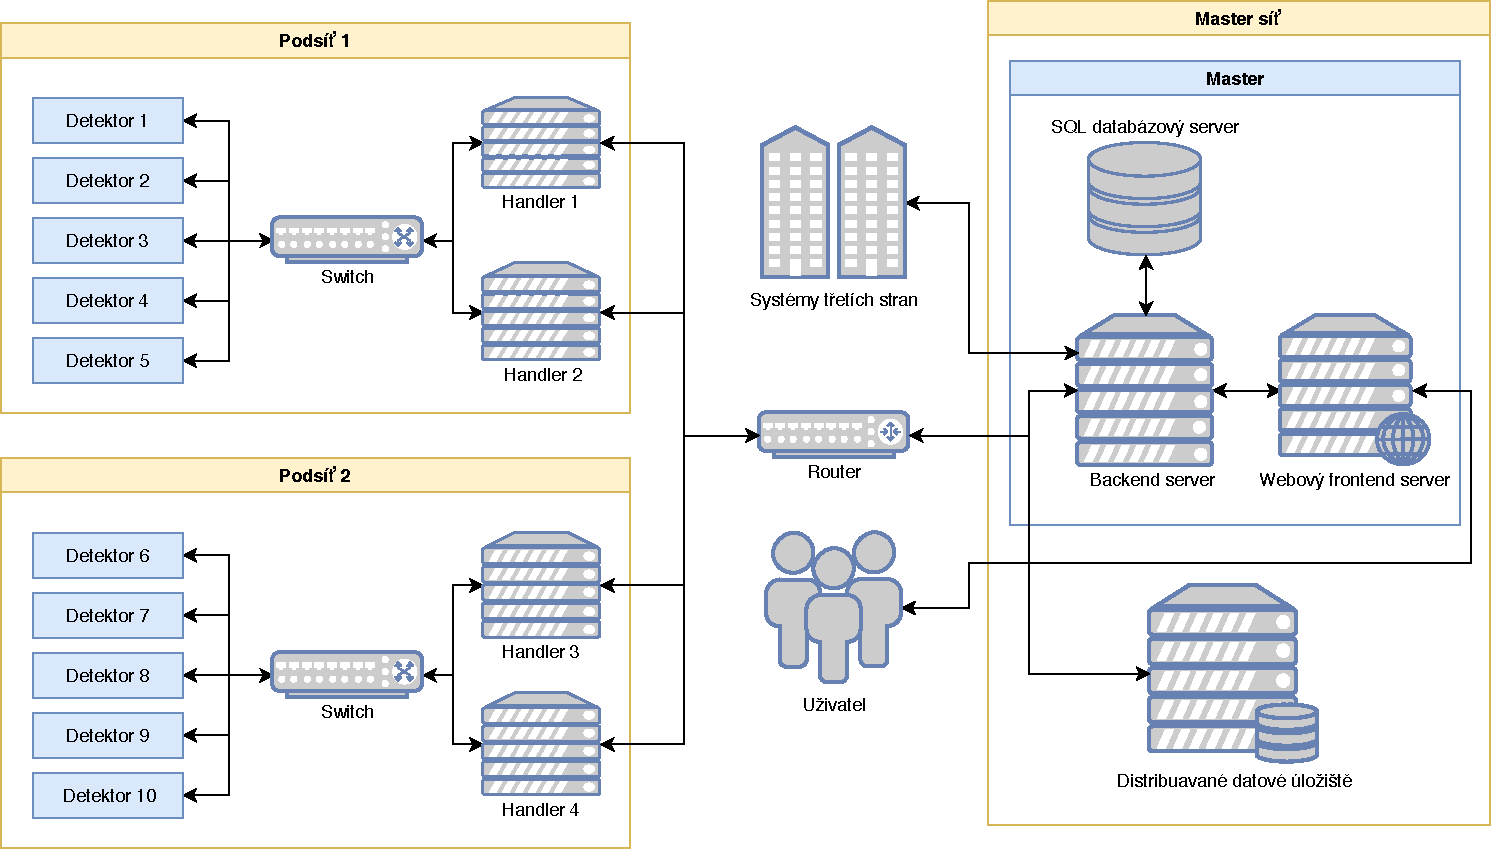
\includegraphics[width=15cm]{figures/arch_hw.pdf}
		\caption{Pixnet: hardwarová architektura s příkladem realizace sítě o dvou podsítích, kde v každé jsou dva handlery a pět detektorů, mastera (s \textit{SQL} databází pro persistenci konfigurace a frontend server poskytující webovou aplikaci) a centrálního datového úložiště naměřených dat.}
		\label{fig:arch:hw_architecture}
	\end{center}
\end{figure}

Master se skládá ze tří komponent:
\begin{description}
    \item[Backend server] implementující business logiku pro komunikaci s handlery (jako například přiřazování detektorů, řízení akvizice dat apod.). Server zároveň poskytuje \textit{API} pro možnou integraci s webovým frontend serverem se systémy třetích stran\footnote{Například pro experiment \textit{ATLAS-TPX} v CERN je plánována integrace s \texttt{DCS} \cite{cern_dcs} (\textit{Detector Control System}), který umožňuje centrální řízení detektorových systému, včetně integrace do bezpečnostního systému \texttt{DSS} (\textit{Detector Safety System}), datového akvizičního systému \texttt{DAQ} (\textit{Data Acquisition System}) apod.}, kterými muže být plnohodnotně řízen.
    \item[Databázový server] poskytující relační \texttt{SQL} databázi pro persistenci konfigurace systému, včetně implementace potřebných rozhraní, stavových informací sítě apod.
    \item[Frontend server] poskytující webovou aplikaci s uživatelským rozhraním pro řízení mastera pomocí jeho \texttt{API}, resp. pro řízení celé sítě.
\end{description}

Na příkladu zmíněném výše je síť využívající jedno centrální datové úložiště. Realizace této komponenty je závislá na poskytnuté implementaci datových rozhraní jednotlivých detektorů. Může být implementovaná pomocí centralizovaného, nebo distribuovaného systému. Umístění úložiště také není omezeno -- může být umístěno v síti mastera, v jednotlivých podsítích, v síti mastera i v jednotlivých podsítích (buffer pro malou šířku pásma spojení podsíť -- master síť), nebo třeba v internetu (cloudové úložiště, jako například \textit{Firebase Firestore}, \textit{Amazon 3S}, \textit{Microsoft Azure} apod.).

%********************************************************************************
% Škálovatelnost
%********************************************************************************
\section{Škálovatelnost}
Škálování systému Pixnet teoreticky není omezeno. Kritickým bodem každého datového akvizičního systému je vyčítání a ukládání naměřených dat. Tento problém je řešen horizontálním škálováním, spočívajícím v přidáváním handlerů, které zajišťují komunikaci s detektory a ukládání naměřených dat.

Možnost škálování datového úložiště je závislá na instanci hardwarové architektury popsané výše. V \cite{gandini2014performance} bylo ukázáno, že \texttt{NoSQL} databázové systémy (jako například \textit{MongoDB} nebo \textit{Apache Cassandra}) jsou dobře horizontálně škálovatelné a jsou schopny zajistit dostatečnou rychlost zápisu vstupních dat. Takže například pro instanci sítě s vhodně zvoleným distribuovaným datovým úložištěm, umístěným v síti mastera (viz obr. \ref{fig:arch:hw_architecture}), budou požadavky na persistenci naměřených dat splněny.

%********************************************************************************
% Použité technologie
%********************************************************************************
\section{Použité technologie}\label{chap:arch:technologie}
V této podkapitole jsou stručně shrnuty technologie použité při implementaci systému.

\begin{description}
    \item[Java] je staticky typovaný, objektově orientovaný programovací jazyk a byl při zahájení implementace zvolen jako primární programovací jazyk pro vývoj tohoto systému. Byl zvolen především pro svou jednoduchost, výkonost a přenositelnost. 
    
    Java je interpretovaný programovací jazyk -- při kompilaci kód není kompilovaný do strojového kódu zvolené platformy, ale do tzv. \textit{bytecode}, který je platformně nezávislý. \textit{Bytecode} pak může být spuštěn na libovolném počítači či zařízení, které disponuje interpretem Javy -- \texttt{JVM} (\textit{Java Virtual Machine}). Java není čistě interpretovaný programovací jazyk, protože v pozdějších verzích byla přidána podpora pro \texttt{JIT} (tzv. \textit{Just-in-time}) kompilátoru, který umožňuje dynamickou kompilaci \textit{bytecode} do strojového kódu dané platformy, díky čemuž může Java ve srovnání s neinterpretovanými programovacími jazyky (\texttt{C++} apod.) dosahovat srovnatelných výsledků.
    
    Java také obsahuje nástroj pro generační správu paměti (tzv. \textit{Garbage Collector}), který se stará o automatické uvolňování paměti mazáním objektů, na které neukazuje žádná reference. Tento nástroj je pro dlouhodobě běžící serverové systémy velice užitečný.

    \item[Kotlin]\label{chap:arch:technologie:kotlin} je moderní staticky typovaný, objektově orientovaný programovací jazyk, který běží nad \texttt{JVM}. Hlavní výhoda Kotlinu je jeho interoperabilita -- kód může být zkompilovaný do Java \textit{bytecode}, do JavaScriptu, nebo i do nativního kódu s tím, že může používat závislosti dané platformy (například pro kompilaci do Java \textit{bytecode} může používat Java knihovny, takže část kompilovaného kódu může být napsána v Javě a část v Kotlinu).

    Oproti Javě poskytuje mnoho výhod, jako například \textit{null-safety} (každá proměnná má kromě svého datového typu i příznak, jestli může být \texttt{null}, což eliminuje spoustu chyb, se kterými se můžeme setkat například v Javě), podpora funkcionálního stylu programování (oproti Javě může být v proměnné uložená funkce), \textit{extension functions} (podobně jako v \texttt{C\#}, je možné přidat funkci do dané třídy bez nutnosti její modifikace, nebo vytvořené poděděné třídy) a další vylepšení. 
    
    Především díky výhodám popsaným výše bylo v pozdější fázi vývoje rozhodnuto o použití Kotlinu, coby primárního programovacího jazyku pro handler a backend mastera. Také bylo experimentováno s použitím Kotlinu pro frontend mastera, pomocí vytvoření společné \textit{code-base} pro backend a frontend mastera (sestávajícího se z business logiky a modelu), ale od tohoto přístupu bylo upuštěno z důvodů omezené podpory kompilátoru Kotlin kódu do JavaScriptu a z důvodu omezené komunitní podpory.
    
    \item[JavaScript] je interpretovaný, objektově orientovaný programovací jazyk, který je zpravidla používán pro tvorbu webových aplikací, ale má i jiná využití. V kontextu webových aplikací, JavaScript kód je interpretován na klientské straně v prohlížeči a pomocí jeho \textit{API} manipuluje s načtenou HTML stránkou, resp. její vnitřní interpretací webovým prohlížečem -- tzv. \texttt{DOM} (\textit{Document Object Model}).
    
    V rámci této práce je použit pro implementaci frontendové části mastera -- webové aplikace poskytující uživatelské rozhraní pro obsluhu systému Pixnet.
     
    \item[Gradle] Je automatizovaný build\footnote{Sestavování počítačových programů.} systém, který vychází z \textit{Apache Ant} a \textit{Apache Maven} a používá \texttt{DSL}\footnote{Z angl. \textit{domain-specific language} (doménově specifický jazyk)} (založeném na \textit{Groovy} a \textit{Kotlin}). Umožňuje automatizované stahování a správu závislostí a knihoven z online repositářů (kromě \textit{Gradle} i \textit{Maven} a \textit{Ivy} pro kompatibilitu s dalšími build systémy).
    
    \item[Spring]\label{chap:arch:technologie:spring} je aplikační framework pro vývoj \texttt{J2EE}\footnote{Označení pro Java \textit{Enterprise Edition} -- platformy pro vývoj podnikových systémů, odvozené od JavaSE (Standard Edition)} aplikací a v rámci systému Pixnet bude použit v rámci implementace handlera a mastera. Spring framework je sada modulů, které nabízejí nástroje jako například webový controller (pro poskytování \texttt{REST API}), \textit{Dependency Injection}\footnote{Technika pro vkládání závislostí mezi komponentami počítačového programu, aniž by v době kompilace měly komponenty na sebe referenci.}, JPA (\textit{Java Persistent API} pro práci s databází), podporu testování apod.

    Novější alternativou je Spring Boot, který je nadstavbou nad původním Spring frameworkem. Spring Boot odstraňuje nutnost komplikovaného definování konfigurace a také přináší možnost zapouzdření do samostatně spustitelné aplikace s embedovaným webovým serverem (\textit{Tomcat}, nebo \textit{Jetty}), takže již není třeba nasazovat \texttt{WAR}\footnote{Z angl. \textit{Web Application Archive} (archív se zkompilovanou webovou \texttt{J2EE} aplikací).} na webový server, protože Spring Boot aplikace je zkompilovatelná do spustitelné \texttt{JAR}\footnote{Z angl. \textit{Java Archive} (archív se zkompilovanou Java aplikací).} aplikace.
    
    \item[ReactJS]\label{chap:arch:technologie:react} je JavaScriptová knihovna pro vývoj uživatelského rozhraní webových aplikací, vyvíjená společností Facebook. React je používán k vývoji tzv. \textit{single-page} aplikací, tj. takových webových aplikací, které k interakci s uživatelem používají jen jednu stránku, jejíž obsah dynamicky přepisují (na rozdíl od stahování nové stránky z webového serveru).
    
    React je založen na principu zapouzdřených komponent, kde každá komponenta má svoje vlastnosti a svůj stav. Komponenty jsou znovupoužitelné a zanořitelné do jiných komponent. Navíc komponenty nepracují přímo s DOM prohlížeče, ale přistupují pouze k jeho virtuální reprezentaci, což umožňuje optimalizovat operace s DOM. Například když nějaká komponenta změní svůj stav (ev. tranzitivně i stav jiných komponent), tak se na stránce přegenerují jen takové komponenty, jejichž stav byl změněn.

    React bude použit pro implementaci frontendové webové aplikace mastera. Vedle Reactu existuje ještě React Native, který je určen pro hybridní vývoj mobilních aplikací, tím se ale v této práci nebudeme zabývat.
    
    \item[PostgreSQL]\label{chap:arch:technologie:postgresql} je nejpoužívanější open source objektově-relační databázový systém. Oproti klasickým relačním databázím (například \textit{MySQL}) má objektově orientovaný databázový model, který je přímo podporován databázovým schématem a dotazovacím jazykem.
    
    Tento databázový systém bude použit pro persistenci konfigurace sítě a bude k němu přistupovat backend mastera.
    
    \item[MongoDB]\label{chap:arch:technologie:mongodb} je \texttt{NoSQL} dokumentový databázový systém. Oproti tradičním relačním databázovým systémům jsou data ukládána do \texttt{BSON}\footnote{Binární forma JSON (z ang. JavaScript Object Notation)} dokumentů. Mezi hlavní výhody \textit{MongoDB} patří:

    \begin{description}
        \item[Indexace:] Na každé pole objektů v dokumentu lze vytvořit index a tím zrychlit vyhledávání v datech.
        \item[Replikace:] \textit{MongoDB} ukládá data do tzv. \textit{replica set}, která obsahuje jednu, nebo více replik dat. Pro případ více replik, jedna vždy funguje jako primární a ostatní jako sekundární, do kterých jsou replikována data z primární repliky. Hlavní výhoda spočívá ve vyšší dostupnosti dat (data lze číst z více replik současně) a spolehlivosti (když jedna replika selže, je nahrazena replikou jinou).
        \item[Horizontální škálování:] \textit{MongoDB} má podporu pro horizontální škálování pomocí tzv. \textit{shardingu} \cite{mongodb-scale}. \textit{Sharded cluster} je pak množina uzlů s jednotlivými \textit{shardy}, kde každý obsahuje podmnožinu \textit{shardovaných} dat.
    \end{description}

\end{description}

\bibliographystyle{csplainnat}

{
%JZ: 11.12.2008 Kdo chce mit v~techto ukazkovych odkazech take odkaz na CSTeX:
\def\CS{$\cal C\kern-0.1667em\lower.5ex\hbox{$\cal S$}\kern-0.075em $}
\bibliography{reference}
}


%%%%%%%%%%%%%%%%%%%%%%%%%% 
% Přílohy
\appendix	

\printnomenclature
\label{apx:zkratky}

\chapter{Obsah přiloženého CD}\label{chap:app:cd}

\definecolor{fblue}{RGB}{92,144,192}
\definecolor{fgreen}{RGB}{34,162,70}

\def\Size{4pt}
\newcommand\myfolder[2][fblue]{%
\begin{tikzpicture}[overlay]
%\begin{scope}[xshift=20pt]
%\tikzset{
\filldraw[draw=folderborder,top color=folderbg!50,bottom color=folderbg]
      (-1.05*\Size,0.2\Size+5pt) rectangle ++(.75*\Size,-0.2\Size-5pt);  
    \filldraw[draw=folderborder,top color=folderbg!50,bottom color=folderbg]
      (-1.15*\Size,-\Size) rectangle (1.15*\Size,\Size);
%\end{scope}  
\end{tikzpicture}%
\makebox[2cm]{\raisebox{-3pt}{{\ttfamily#2}}}%
%}
}


\begin{figure}[th!]
\begin{center}
\begin{forest}
  for tree={
    font=\ttfamily,
    grow'=0,
    child anchor=west,
    parent anchor=south,
    anchor=west,
    calign=first,
    inner xsep=7pt,
    edge path={
      \noexpand\path [draw, \forestoption{edge}]
      (!u.south west) +(7.5pt,0) |- (.child anchor) \forestoption{edge label};
    },
    before typesetting nodes={
      if n=1
        {insert before={[,phantom]}}
        {}
    },
    fit=band,
    before computing xy={l=15pt},
  }  
[CD/
	[pixnet/
		[commons/ - modul se společnými závislosti]
		[detector\_communication\_intf/ - modul s komunikačním interface]
		[detector\_communication\_katherine/ - komunikační modul Katherine]
		[detector\_data\_persistence\_intf/ - modul s datovým interface]
		[handler/ - modul s handlerem]
		[katherine\_commons/ - společné závislosti Katherine modulů]
		[katherine\_emulator/ - emulátor Katherine]
		[katherine\_persistence\_file/ - datový modul Katherine]
		[master/ - modul s backendovou aplikací mastera]
	]
	[pixnet\_frontend/ - webová single-page aplikace]
	[text/
		[src/ - adresář se zdrojovými soubory tohoto dokumentu]
		[master-thesis-jakub-begera-2019.pdf - tato práce ve formátu PDF]
		[abstract\_cz.txt - abstrakt česky]
		[abstract\_en.txt - abstrakt anglicky]
	]
	[detector\_model.json - přehled příkazů komunikačního modulu Katherine]
]
\end{forest}
\end{center}
\caption{Obsah přiloženého CD}
\label{fig:attached-cd}
\end{figure}

\end{document}
